\documentclass[11pt, a4paper]{article}
\usepackage[utf8]{inputenc}
\usepackage[T1]{fontenc}
\usepackage[frenchb]{babel}
\usepackage[top=3cm, bottom=3cm, left=2cm, right=2cm]{geometry}
\usepackage{listings}
\usepackage{graphicx}
\usepackage{fancyhdr}
\usepackage{hyperref}
\usepackage{float}
\usepackage{amsmath}
\usepackage{amsthm}
\usepackage{amssymb}
\usepackage{mathrsfs}
\usepackage{mathrsfs}
\usepackage{dsfont}
\usepackage{fourier-orns}
\usepackage[linesnumbered, ruled, french]{algorithm2e}
\usepackage{tabularx}
\usepackage{tabularx,ragged2e,booktabs,caption}
\usepackage{tikz}

\newcommand{\hmark}{\rule{\linewidth}{0.5mm}}

% pour faciliter l'écriture de la somme en dehors des \[\]
\newcommand{\somme}[2]{\underset{#1}{\overset{#2}{\sum}}}

\definecolor{one}{HTML}{F0F4FE}
\definecolor{two}{HTML}{C5E0FF}
\definecolor{three}{HTML}{81C1FF}
\definecolor{four}{HTML}{598AF3}
\definecolor{five}{HTML}{0071C4}

\begin{document}
\begin{titlepage}
\pagenumbering{gobble}

\centering

\begin{figure}[t]
\begin{center}

\includegraphics[width=8cm]{Images/upmc.png}
\end{center}
\end{figure}

\hmark \\[0.5cm]
\textsc{\textbf{\Large Deux algorithmes pour l'identification d'un axe gauche-droite sur les candidats à une élection}} \\[0.5cm]
\textsc{P-ANDROIDE} \\[0.5cm]
\hmark \\[5cm]

\begin{minipage}{0.4\textwidth}
\begin{flushleft}
Thibault \textsc{Gigant}\\
Laura \textsc{Greige}
\end{flushleft}
\end{minipage}
~
\begin{minipage}{0.4\textwidth}
\begin{flushright} \large
\emph{Encadrant :}\\
Olivier \textsc{Spanjaard}
\end{flushright}
\end{minipage}\\[4cm]

\large Année 2015 - 2016

\end{titlepage}
\newpage

\tableofcontents

\newpage

\pagenumbering{arabic}

\pagestyle{fancy}
\renewcommand{\headrulewidth}{1pt}
\lhead{\textbf{P-ANDROIDE -- Choix Social Computationnel}}

\section*{Introduction}
\addcontentsline{toc}{section}{Introduction}

Habituellement, lors d'un vote, l'\'{e}lecteur est amen\'{e} \`{a} choisir un unique candidat parmi une multitude. Lorsqu'il est donn\'{e} la possibilit\'{e} aux \'{e}lecteurs de ne plus voter pour un seul candidat, mais pour un sous-ensemble d'entre eux qu'il approuverait, on parle de vote par \og approbation \fg{}, ou vote par \og assentiment\fg{}. Avec cette proc\'{e}dure de vote, on peut \'{e}tudier les diff\'{e}rents votes formul\'{e}s pour tenter d'en extraire un axe \og gauche-droite \fg{} classant les candidats les uns par rapport aux autres en fonction de leur proximit\'{e} dans les bulletins r\'{e}colt\'{e}s.

Afin de r\'{e}soudre ce probl\`{e}me, deux principales m\'{e}thodes seront utilis\'{e}es dans ce projet :
\begin{itemize}
\item Un algorithme de s\'{e}riation permettant de calculer un axe en fonction des similarit\'{e}s entre les candidats, calculées à partir des bulletins de vote.
\item Un algorithme de branch \& bound identifiant un sous-ensemble le plus large possible de bulletins coh\'{e}rents avec un axe. Un bulletin est dit cohérent avec un axe s'il correspond à un sous-ensemble de candidats contigus sur cet axe.\\
\end{itemize}

Ces deux approches seront plus amplement d\'{e}taill\'{e}es dans la seconde partie de ce rapport. La premi\`{e}re partie quant \`{a} elle d\'{e}taillera les diff\'{e}rentes t\^{a}ches qui ont \'{e}t\'{e} demand\'{e}es par l'encadrant. La troisi\`{e}me partie concernera l'impl\'{e}mentation en elle-m\^{e}me, le logiciel cr\'{e}\'{e} pour r\'{e}pondre \`{a} ces t\^{a}ches. Enfin, une derni\`{e}re partie donnera les r\'{e}sultats de tests numériques sur des donn\'{e}es r\'{e}elles.

\section{Cahier des Charges}

Deux approches ont donc \'{e}t\'{e} demand\'{e}es, la premi\`{e}re \'{e}tant une approche par s\'{e}riation et la seconde par branch \& bound. De plus, une interface graphique pour lancer les algorithmes et visualiser les r\'{e}sultats a \'{e}t\'{e} requise.

\subsection{S\'{e}riation}
\label{cdc_seriation}

La premi\`{e}re m\'{e}thode qui sera utilis\'{e}e appliquera un algorithme de s\'{e}riation. Le principe est de calculer une matrice dont l'élément en position $ij$ repr\'{e}sente la dissimilarit\'{e} entre le candidat $i$ et le candidat $j$. L'indice de dissimilarité peut \^{e}tre calcul\'{e} de plusieurs mani\`{e}res, et chacune sera \'{e}tudi\'{e}e et compar\'{e}e aux autres, pour d\'{e}terminer laquelle correspond le plus \`{a} la recherche de l'axe voulu. L'indice est un r\'{e}el compris entre 0 et 1, tel que 0 repr\'{e}sente une similarit\'{e} parfaite, et 1 une dissimilarit\'{e} totale. Bien entendu, la matrice de dissimilarité est parfaitement sym\'{e}trique et a pour diagonale principale des 0. Elle peut donc \^{e}tre consid\'{e}r\'{e}e comme une matrice triangulaire sup\'{e}rieure stricte, puisque la diagonale ne changera pas et la partie inf\'{e}rieure n'est que le miroir de la partie sup\'{e}rieure.

A partir de cette matrice, pour trouver un axe sur les candidats, il suffit alors de trouver une permutation des candidats (donc des lignes et des colonnes) telle que les \'{e}l\'{e}ments sur les lignes et les colonnes soient croissants au fur et \`{a} mesure que l'on s'\'{e}loigne de la diagonale. Du moins, on cherche à être le plus proche possible de cette propriété. On peut procéder de deux manières pour ce faire :\\

\begin{itemize}
\item  \textbf{la force brute} ~  considère toutes les permutations possibles, donc tous les axes possibles, calcule un score \`{a} partir de la matrice de dissimilarit\'{e} de chaque permutation, et renvoie celle donnant le score minimal. Cette m\'{e}thode na\"{i}ve sera impl\'{e}ment\'{e}e, mais \'{e}tant donn\'{e}e sa complexit\'{e} exponentielle, puisqu'elle demande de calculer le score des $n!$ axes possibles ($n$ \'{e}tant le nombre de candidats), elle ne sera utilis\'{e}e que pour v\'{e}rifier la validit\'{e} de la solution suivante, avec un nombre de candidats restreint.\\

\item \textbf{la procédure de programmation dynamique} ~ est inspir\'{e}e des travaux de \textsc{Hubert} \cite{huberDynamic}. Elle permet d'identifier une permutation optimale en $O(2^n)$, où $2^n$ est le nombre de sous-ensembles possibles de candidats. Cela reste conséquent, mais largement inférieur à $n!$.
\end{itemize}

\subsection{Branch \& bound}

Pour d\'{e}terminer un axe compatible avec un nombre maximum de votants, on fait appel \`{a} une proc\'{e}dure de branch \& bound. Supposons qu'on ait $n$ bulletins distincts. Un algorithme d'\'{e}num\'{e}ration compl\`{e}te des solutions peut \^{e}tre illustr\'{e} par une arborescence de hauteur $n$, o\`{u} en chaque n\oe{}ud on d\'{e}cide de s\'{e}lectionner ou non un bulletin. On obtient donc un arbre \`{a} $2^{n}$ feuilles, et en chacune de ces feuilles, on a une solution possible qui correspond \`{a} un sous-ensemble de bulletins. On cherche s'il existe un axe compatible avec l'ensemble des bulletins s\'{e}lectionn\'{e}s et on retient la meilleure solution obtenue, c'est-\`{a}-dire l'ensemble le plus large de bulletins coh\'{e}rents avec un m\^{e}me axe.

Afin d'am\'{e}liorer l'efficacit\'{e} du branch \& bound, seules les solutions potentiellement de bonne qualit\'{e} seront \'{e}num\'{e}r\'{e}es, les solutions ne pouvant pas conduire \`{a} am\'{e}liorer la solution courante ne seront pas explor\'{e}es.\\

Le branch \& bound est bas\'{e} sur trois principes : le principe de s\'{e}paration qui consiste \`{a} s\'{e}parer un ensemble de solutions en sous-ensembles, le principe d'\'{e}valuation qui permet de conna\^{i}tre la qualit\'{e} des n\oe{}uds \`{a} traiter, et le principe du parcours de l'arbre qui permet de choisir le prochain n\oe{}ud \`{a} s\'{e}parer.

\subsection{Interface graphique}

L'interface demand\'{e}e est une interface simple, permettant d'abord de choisir l'algorithme \`{a} appliquer, avec quelles caract\'{e}ristiques, et sur quels fichiers. Deux modes ont d\^{u} \^{e}tre impl\'{e}ment\'{e}s. L'un permet de r\'{e}aliser des bancs d'essai, donnant des r\'{e}sultats d\'{e}taill\'{e}s pour tous les fichiers s\'{e}lectionn\'{e}s. L'autre est plus interactif, et affichera pour chaque instance un graphe refl\'{e}tant les diff\'{e}rences, s'il y en a, entre le ou les axes trouv\'{e}s par l'algorithme et l'axe \og r\'{e}el \fg{}, r\'{e}cup\'{e}r\'{e} manuellement depuis un site tel que \href{www.wikipedia.fr}{Wikipedia}.

\section{Analyse et conception}
Nous détaillons dans cette partie les deux algorithmes implémentés : la sériation et le branch \& bound.

\subsection{S\'{e}riation}

Le premier algorithme \`{a} impl\'{e}menter est un algorithme par s\'{e}riation. La s\'{e}riation est la capacit\'{e} \`{a} comparer deux entit\'{e}s pour les ranger dans un ordre pr\'{e}cis. Par exemple dire qu'un objet est plus grand qu'un autre ou inversement. Dans le cas du probl\`{e}me pos\'{e}, le but est de positionner les candidats les uns par rapport aux autres sur un axe gauche-droite en fonction des bulletins exprim\'{e}s. En effet, il para\^{i}t normal que deux candidats souvent pr\'{e}sents dans un m\^{e}me bulletin ne soient pas trop \'{e}loign\'{e}s l'un de l'autre dans l'axe.

\subsubsection{Principe}

La m\'{e}thode emploie une matrice symbolisant la dissimilarit\'{e} entre les candidats. Comme expliqué précédemment (\ref{cdc_seriation}) on a donc une matrice carr\'{e}e, o\`{u} chaque ligne et chaque colonne repr\'{e}sente un candidat. Le calcul de la dissimilarit\'{e} peut se faire de diff\'{e}rentes façons. Nous noterons, pour chaque bulletin $b_k$, le nombre de personnes $n_k$ ayant voté de cette manière. De plus, nous noterons $b_{i \wedge j}$ les bulletins contenant les candidats $i$ et $j$, $b_{i \vee j}$ les bulletins contenant le candidat $i$ ou le candidat $j$, et $d_{ij}$ la dissimilarité entre ces deux candidats. Pour ce projet, 3 grandes fonctions ont \'{e}t\'{e} utilis\'{e}es pour mod\'{e}liser la dissimilarit\'{e} entre deux candidats :

\medskip
\begin{itemize}
\item En comptant le nombre de bulletins sur lesquels les deux candidats sont pr\'{e}sents, divis\'{e} par le nombre de bulletins totaux. Pour obtenir un indice de dissimilarité, il suffit de retrancher ce r\'{e}sultat \`{a} 1 :
\[
\forall i, j\text{ candidats, } d_{ij} = 1 - \dfrac{\somme{b_{i \wedge j}}{} n_{i \wedge j}}{\somme{b_k}{} n_k}
\]
Nous appellerons cette fonction de dissimilarité \texttt{dissimilarity\_and\_n} par la suite.

\medskip
\item En comptant le nombre de bulletins sur lesquels les deux candidats sont pr\'{e}sents, divis\'{e} par le nombre de bulletins o\`{u} l'un ou l'autre des candidats est pr\'{e}sent. De m\^{e}me, il suffit de retrancher ce r\'{e}sultat \`{a} 1 pour obtenir la dissimilarit\'{e} entre les deux candidats :
\[
\forall i, j\text{ candidats, } d_{ij} = 1 - \dfrac{\somme{b_{i \wedge j}}{} n_{i \wedge j}}{\somme{b_{i \vee j}}{} n_{i \vee j}}
\]
Nous appellerons cette fonction de dissimilarité \texttt{dissimilarity\_and\_or} par la suite.

%\item En sommant l'inverse du nombre de personnes ayant vot\'{e} pour chaque bulletin approuvant les deux candidats, divis\'{e} par la somme des inverses du nombre de personnes ayant vot\'{e} pour chaque bulletin approuvant l'un ou l'autre des candidats :
\medskip
\item Il est aussi possible de prendre en compte la taille des bulletins. En effet, il semble naturel de donner plus de poids à un bulletin ou seulement deux candidats sont présents, plutôt qu'à un bulletin où ces deux candidats sont noyés sous beaucoup d'autres. Ainsi, en s'inspirant de la formule précédente, et en notant $\vert b_k \vert$ le nombre de candidats approuvés dans le bulletin $b_k$ :
\[
\forall i, j\text{ candidats, } d_{ij} = 1 - \dfrac{\somme{b_{i \wedge j}}{} \dfrac{1}{\vert b_{i \wedge j} \vert} \times n_{i \wedge j}}{\somme{b_{i \vee j}}{} \dfrac{1}{\vert b_{i \vee j}\vert} \times n_{i \vee j}}
\]
Nous appellerons cette fonction de dissimilarité \texttt{dissimilarity\_over\_over} par la suite.
\end{itemize}

\bigskip
Pour obtenir l'axe gauche-droite qui nous int\'{e}resse, il faut trouver une permutation sur les lignes et les colonnes (la m\^{e}me permutation sur les lignes et les colonnes), telle que les valeurs des dissimilarit\'{e}s soient croissantes lorsqu'on s'\'{e}loigne de la diagonale. On appelle une matrice respectant cette propriété une matrice \og Anti-Robinson \fg{}.

On cherche à transformer la matrice ainsi pour la raison suivante. Prenons par exemple 3 candidats $i, j, k$, positionnés dans ce même ordre dans l'axe gauche-droite trouvé. La dissimilarité entre le candidat $i$ et le candidat $k$, comme la matrice possède cette propriété, sera supérieure à celle entre les candidats $i$ et $j$, ou celle entre les candidats $j$ et $k$. Voici un petit schéma pour illustrer ces propos :

\begin{center}
\begin{minipage}{0.4\textwidth}
\setlength{\unitlength}{1cm}
\begin{picture}(4,2)(-1,-1)
% axe x
   \put(0,0){\vector(1,0){4}}
   \multiput(1,-0.2)(1,0){3}{\line(0,1){0.4}} % traits de graduation
   \put(0.9,-0.6){i} % valeurs graduées
   \put(1.9,-0.6){j}
   \put(2.9,-0.6){k}
\end{picture}
\end{minipage}
\begin{minipage}{0.1\textwidth}
$\Longleftrightarrow$
\end{minipage}
\begin{minipage}{0.4\textwidth}
$d_{ik} \geq \max \{d_{ij}, d_{jk}\}$
\end{minipage}
\end{center}

On aura donc ainsi trouvé l'axe qui positionne les candidats les plus similaires les uns à côté des autres.

En pratique, il n'est que rarement possible d'obtenir une matrice de dissimilarité parfaitement Anti-Robinson. C'est pourquoi on se ramène à un problème d'optimisation en définissant une \og distance \fg{} à la propriété souhaitée. On attribue alors pour chaque permutation des lignes et colonnes un score \`{a} cette matrice. Dans ce projet, nous avons envisagé deux manières de calculer ce score.

Pour chacune, on regarde chaque \'{e}l\'{e}ment $d_{ij}$ $(j > i)$, de la partie sup\'{e}rieure droite de la matrice. Pour rappel, il est inutile de travailler sur la partie inférieure gauche, car elle est symétrique à la partie supérieure. On s'éloigne alors de la propriété voulue si il existe des éléments $d_{ik}$ et $d_{ij}$ $(k>j)$ sur la même ligne tels que $d_{ik} < d_{ij}$. De même, il faut regarder sur les colonnes s'il existe des éléments $d_{kj}$ et $d_{ij}$ $(k<i)$ tels que $d_{kj} < d_{ij}$. En notant $n$ le nombre de candidats, les deux manières de calculer le score $s$ d'une matrice de dissimilarité sont les suivantes :\\

\begin{itemize}
\item \textbf{Score non-pond\'{e}r\'{e}e :} on ajoute 1 au score à chaque fois qu'on s'éloigne de la propriété. On a donc :
\[
s = \somme{i = 0}{n} \somme{j = i+1}{n} \somme{k = j+1}{n} \mathds{1}_{d_{ik} < d_{ij}}+ \somme{i = 1}{n} \somme{j = 0}{i-1} \somme{k = 0}{j-1} \mathds{1}_{d_{kj} < d_{ij}}
\]

\item \textbf{Score pond\'{e}r\'{e} :} cette fois, on prend en compte l'écart qu'il y a entre les éléments qui ne vérifient pas la propriété :
\[
s = \somme{i = 0}{n} \somme{j = i+1}{n} \somme{k = j+1}{n} [\mathds{1}_{d_{ik} < d_{ij}} \times (d_{ij} - d_{ik})]+ \somme{i = 1}{n} \somme{j = 0}{i-1} \somme{k = 0}{j-1} [\mathds{1}_{d_{kj} < d_{ij}} \times (d_{ij} - d_{kj})]
\]

\end{itemize}

Plus le score est proche de 0, plus on est proche d'une matrice Anti-Robinson. On a alors une permutation donnant un axe gauche-droite compatible avec les bulletins exprimés. Bien entendu, lorsqu'on trouve une permutation donnant un score minimal, la permutation avec les candidats dans l'ordre inverse donnera un score identique. En effet, cette permutation inverse donnera la matrice transpos\'{e}e \`{a} la premi\`{e}re, et donc les incoh\'{e}rences rep\'{e}r\'{e}es dans le colonnes de l'une seront rep\'{e}r\'{e}es dans les lignes de l'autre, et inversement. C'est pourquoi il y a toujours un nombre pair d'axes compatibles avec les donn\'{e}es.\\

Rappelons que la force brute requerrait le calcul du score de $n!$ matrices, $n$ \'{e}tant le nombre de candidats du scrutin. Il faut de plus prendre en compte le temps n\'{e}cessaire pour appliquer les permutations \`{a} la matrice.

Nous avons donc implémenté une procédure de programmation dynamique proposée par \textsc{Hubert} et \textsc{Golledge} \cite{huberDynamic}. Elle repose sur le postulat suivant : en partant de $n$ candidats, si on arrive \`{a} classer de façon certaine $n-1$ candidats à gauche dans l'axe, il ne reste plus qu'\`{a} placer le dernier candidat \`{a} droite des autres. On r\'{e}alise donc d'abord un appel r\'{e}cursif pour placer correctement les $n-1$ candidats, puis on place le dernier.

%Cependant, pour \^{e}tre s\^{u}r de placer le bon candidat à l'extrêmité, il est n\'{e}cessaire d'appliquer cet algorithme en plaçant chaque candidat à droite des autres. Après appel récursif sur les candidats restants, on peut comparer le score de la matrice de dissimilarité associée à chaque permutation trouvée. Il faut donc effectuer $n$ appels r\'{e}cursifs au départ lorsqu'on a $n$ candidats.

Pour expliquer cela plus clairement, on notera $s$ la fonction donnant le score minimal d'un sous-ensemble de candidats, c'est à dire le score retourné par la fonction sériation correspondant à ce sous-ensemble. De même, on notera $h$ la fonction donnant la distance entre un candidat $c_i$ et un sous-ensemble. Avec $C$ l'ensemble des $n$ candidats, la relation de récurrence s'écrit :
\[
s(C) = \min_{c_i \in C} [s(C \setminus c_i) + d(C \setminus c_i, c_i)]
\]

\subsubsection{Pseudo-Code}

\noindent Voici ci-dessous le pseudo-code pour la programmation dynamique. L'algorithme prend en entrée la matrice de dissimilarit\'{e} calcul\'{e}e de la mani\`{e}re souhait\'{e}e, l'ensemble entier des candidats, et un dictionnaire vide qui sera rempli par l'algorithme :\\

\begin{algorithm}[H]
	\caption{S\'{e}riation}
	\Entree{
		\par\leftskip=1.5em Matrice de similarit\'{e} $mat$\\
		\par\leftskip=1.5em Ensemble des candidats impliqu\'{e}s $candidates\_set$\\
		\par\leftskip=1.5em Dictionnaire des r\'{e}sultats d\'{e}j\`{a} calcul\'{e}s $function\_map$ dont les cl\'{e}s sont les sous-ensembles de candidats et les valeurs sont des tuples donnant le score et les permutations optimales associ\'{e}es.
	}
	\Sortie{
	    \par\leftskip=1.5em Dictionnaire des r\'{e}sultats pour chaque sous-ensemble de candidats : $function\_map$
	}
	
	\bigskip
	\Deb{
		\Si{$candidates\_set$ a d\'{e}j\`{a} \'{e}t\'{e} calcul\'{e}}{
		    \Retour{$function\_map$}
		}
		
		$n$ := cardinalit\'{e} de $candidates\_set$
		
		\Si{n = 1}{
		    $function\_map[candidates\_set] := (0, candidates\_set)$\\
		    \Retour{$function\_map$}
		}
		
		$temp$ := []
		
		\Pour{chaque combinaison de n-1 candidats dans candidates\_set}{
		    $candidat\_courant := candidates\_set \setminus combinaison$\\
		    $function\_map :=$ S\'{e}riation$(mat, combinaison, function\_map)$\\
		    $scores :=$ distance$(similarity\_matrix, combinaison, candidat\_courant, function\_map)$\\
		    \# La fonction distance renvoie une liste de tuples scores
		    
		    \Pour{chaque score dans scores}{
		        Ajout de $(score[0] + function\_map[combinaison][0], score[1])$ \`{a} temp
		    }
		}
		
		On ne garde dans temp que les tuples avec le score minimum
		
		$score\_min :=$ score minimal dans temp
		
		$liste\_combinaisons :=$ liste des combinaisons donnant le score minimum dans temp
		
		$function\_map[candidates\_set] := (score\_min, liste\_combinaisons)$
		
		\Retour{$function\_map$}
	}
	
\end{algorithm}

\bigskip

Dans cet algorithme, la fonction distance a \'{e}t\'{e} introduite. Cette fonction calcule la distance de la matrice au fait d'être Anti-Robinson, du moins en partie, en fonction du positionnement du candidat courant apr\`{e}s les candidats présents dans $candidates\_set$. En effet, une fois qu'on a positionné le candidat le plus à gauche, quelle que soit la permutation des candidats suivants, on peut déjà calculer l'impact de ce positionnement sur le score de la matrice. La colonne et la ligne de ce candidat étant positionnées de façon certaine, on peut regarder les éléments à droite de cette colonne et en haut de cette ligne qui ne permettraient pas à la matrice d'être Anti-Robinson. C'est donc bien le score de la matrice qui est calculé, mais uniquement par rapport à une ligne et une colonne qu'on suppose bien placée. Il faut donc réitérer le processus une fois qu'on aura placé le second candidat en rajoutant le score obtenu après placement du premier, puis le troisième, et ainsi de suite. Au final, on aura bien le score final de la matrice, donnant son éloignement à la propriété recherchée.

% C'est d'ailleurs \`{a} ce niveau l\`{a} qu'il est faite la diff\'{e}rence de calcul du score entre les syst\`{e}mes pond\'{e}r\'{e} et non-pond\'{e}r\'{e} d\'{e}crits pr\'{e}c\'{e}demment. Effectivement, on compare bien les éléments entre eux pour regarder à quel point on s'éloigne d'une matrice Anti-Robinson.\\

Une fois l'algorithme de s\'{e}riation appliqu\'{e}, il ne reste plus qu'\`{a} retourner les axes les plus coh\'{e}rents avec les bulletins, ainsi que le score de la matrice engendr\'{e}e par ces axes. Ces deux sorties sont stock\'{e}es dans le dictionnaire $function\_map$.% dans la valeur correspondant \`{a} l'ensemble des candidats.

\bigskip
Voici un exemple trivial, à trois candidats $C_1, C_2, C_3$, décrivant comment trouver une permutation donnant un score minimal. On notera $s$ la fonction donnant le score minimal d'un sous-ensemble de candidats, c'est à dire le score retourné par la fonction sériation correspondant à ce sous-ensemble. De même, on notera $h$ la fonction donnant la distance entre un candidat et un sous-ensemble, distance calculée de façon pondérée pour cet exemple. Pour ce faire, nous donnerons une matrice de dissimilarité fictive simple, constituée d'entiers en lieu et place des flottants entre 0 et 1, pour faciliter les calculs : 

\begin{center}
$\bordermatrix{
& C_1 & C_2 & C_3 \cr
C_1 & 0 & 3 & 1 \cr
C_2 & 3 & 0 & 2 \cr
C_3 & 1 & 2 & 0}
~
\bordermatrix{
& C_1 & C_3 & C_2 \cr
C_1 & 0 & 1 & 3 \cr
C_3 & 1 & 0 & 2 \cr
C_2 & 3 & 2 & 0}
~
\bordermatrix{
& C_2 & C_1 & C_3 \cr
C_2 & 0 & 1 & 2 \cr
C_1 & 1 & 0 & 3 \cr
C_3 & 2 & 3 & 0}$

\vspace{0.5cm}

$\bordermatrix{
& C_2 & C_3 & C_1 \cr
C_2 & 0 & 2 & 3 \cr
C_3 & 2 & 0 & 1 \cr
C_1 & 3 & 1 & 0}
~
\bordermatrix{
& C_3 & C_1 & C_2 \cr
C_3 & 0 & 1 & 2 \cr
C_1 & 1 & 0 & 3 \cr
C_2 & 2 & 3 & 0}
~
\bordermatrix{
& C_3 & C_2 & C_1 \cr
C_3 & 0 & 2 & 1 \cr
C_2 & 2 & 0 & 3 \cr
C_1 & 1 & 3 & 0}
$\\[0.5cm]
\end{center}

La recherche d'un axe gauche droite sur cet exemple donnerait :
\begin{equation*}
\begin{aligned}
    &s(\{C_1\}) = 0\\
    &s(\{C_2\}) = 0\\
    &s(\{C_3\}) = 0\\
\end{aligned}
\end{equation*}

\begin{equation*}
\begin{aligned}
    s(\{C_1, C_2\}) &= &\min \{&s(\{C_1\}) + d(\{C_1\}, C_2), s(\{C_2\}) + d(\{C_2\}, C_1)\}\\
    &= &\min \{&0 + ((3-1) + (2-1)), 0 + (3-2)\} = 1\\[0.5cm]
    s(\{C_1, C_3\}) &= &\min \{&s(\{C_1\}) + d(\{C_1\}, C_3), s(\{C_3\}) + d(\{C_3\}, C_1)\}\\
    &= &\min \{&0 + 0, 0 + (3-2)\} = 0\\[0.5cm]
    s(\{C_2, C_3\}) &= &\min \{&s(\{C_2\}) + d(\{C_2\}, C_3), s(\{C_3\}) + d(\{C_3\}, C_2)\}\\
    &= &\min \{&0 + 0, 0 + ((2-1) + (3-1))\} = 0\\[0.5cm]
    s(\{C_1,C_2,C_3\}) &= &\min \{&s(\{C_1, C_2\}) + d(\{C_1, C_2\}, C_3),\\
    &&&s(\{C_1,C_3\}) + d(\{C_1,C_3\}, C_2),\\
    &&&s(\{C_2, C_3\}) + d(\{C_2, C_3\}, C_1)\}\\
    &= &\min \{&1 + 0,\ 0 + 0,\ 0 + 0\} = 0\qquad\quad
\end{aligned}
\end{equation*}

\bigskip
On peut alors retrouver les permutations optimales par induction arrière depuis le résultat donné par $s(\{C_1,C_2,C_3\})$. Ici il y a deux possibilités, donnant deux axes symétriques, ce qui est normal, comme expliqué précédemment. On a déterminé que les permutations optimales sont les suivantes : $C_1C_3C_2$ et $C_2C_3C_1$.

\subsection{Branch \& bound}

Le deuxi\`{e}me algorithme impl\'{e}ment\'{e} est un algorithme par s\'{e}paration et \'{e}valuation. Le Branch \& bound est une m\'{e}thode arborescente qui consiste \`{a} \'{e}num\'{e}rer les solutions r\'{e}alisables en \'{e}liminant les solutions partielles qui ne m\`{e}nent pas \`{a} la solution que l'on recherche. En effet, on cherche un sous-ensemble de bulletins coh\'{e}rents, il est donc n\'{e}cessaire de formaliser cette coh\'{e}rence avant de passer \`{a} l'algorithme de Branch \& Bound.

\subsubsection{Formalisation}
\label{1consecutifs}

Pour trouver un sous-ensemble $S$ de bulletins coh\'{e}rents, il suffit de trouver un axe compatible avec les bulletins pr\'{e}sents dans $S$. En effet, s'il existe un tel axe, alors pour tout bulletin $b$ appartenant à $S$, $b$ figure dans l'axe et est un sous-ensemble contigu de l'axe. C'est la propri\'{e}t\'{e} des 1-cons\'{e}cutifs : soit une matrice binaire dont chaque ligne repr\'{e}sente un bulletin et chaque colonne repr\'{e}sente un candidat. La matrice $M$ est alors compos\'{e}e de 0 et de 1, $m_{ij} = 1$ si le votant $i$ approuve le candidat $j$, $m_{ij} = 0$ sinon. Si l'on trouve une permutation des colonnes telle que les 1 de la matrice sont cons\'{e}cutifs sur chaque ligne, alors on a trouv\'{e} un axe compatible.\\

Exemple : Prenons comme exemple un ensemble de bulletins $S = \{\{1,2,3\},\{1,3\},\{3,4\}, \{1,3,4\}$\} pour les candidats 1, 2, 3 et 4. On trouve la matrice suivante :\\

\begin{center}
$\bordermatrix{
& 1 & 2 & 3 & 4 \cr
\{1,2, 3\} ~~~~ & 1 & 1 & 1 & 0 \cr
\{1,3\} & 1 & 0 & 1 & 0 \cr
\{3,4\} & 0 & 0 & 1 & 1 \cr
\{1,3,4\} & 1 & 0 & 1 & 1}
%
\implies
%
\bordermatrix{
& 2 & 1 & 3 & 4 \cr
\{1,2, 3\} ~~~~ & 1 & 1 & 1 & 0 \cr
\{1,3\} & 0 & 1 & 1 & 0 \cr
\{3,4\} & 0 & 0 & 1 & 1 \cr
\{1,3,4\} & 0 & 1 & 1 & 1}$\\[0.8cm]
\end{center}

Les 1 de la matrice de droite sont tous cons\'{e}cutifs sur chacune des lignes avec la permutation $p = [2,1,3,4]$, on a donc trouv\'{e} un axe compatible qui est $a = 2-1-3-4$. On peut donc dire que les bulletins sont coh\'{e}rents.\\

D'autre part, pour tester si un bulletin est coh\'{e}rent avec un sous-ensemble de bulletins, il faut v\'{e}rifier qu'il est compatible avec au moins un des axes trouv\'{e}s pour le sous-ensemble. Dans l'exemple pr\'{e}c\'{e}dent, un seul axe \'{e}tait compatible avec le sous-ensemble $S$, donc pour tester la coh\'{e}rence d'un nouveau bulletin avec ce sous-ensemble, il suffit de tester la coh\'{e}rence entre le nouveau bulletin et l'axe trouv\'{e}. Soit deux bulletins $b_{1} = \{2,1\}$ et $b_{2} = \{2,3\}$ : $b_{1}$ est compatible avec l'axe $a$ puisque 1 et 2 se trouvent c\^{o}te \`{a} c\^{o}te dans l'axe, alors que le bulletin $b_{2}$ ne l'est pas.

Prenons un autre exemple où plusieurs axes diff\'{e}rents sont compatibles avec un même sous-ensemble de bulletins. Soit $S' = \{\{1,2,3\}, \{2,3,4\}\}$ un sous-ensemble de bulletins. Les axes compatibles avec $S'$ sont $a_{1} = 1-2-3-4$ et $a_{2} = 4-2-3-1$. Soit un bulletin $b_{3} = \{1,3\}$ : $b_{3}$ n'est pas coh\'{e}rent avec $a_{1}$, mais il l'est avec $a_{2}$. Il est donc coh\'{e}rent avec le sous-ensemble de bulletins $S'$.\\

On en d\'{e}duit qu'il est bien n\'{e}c\'{e}ssaire d'\'{e}num\'{e}rer tous les axes compatibles avec un sous-ensemble pour tester la coh\'{e}rence d'un nouveau bulletin avec celui-ci.

\subsubsection{Algorithme}

On note $C = \{c_{1}, c_{2}, ..., c_{m}\}$ l'ensemble des $m$ candidats impliqu\'{e}s et $L = \{(x_{1}, b_{1}), (x_{2}, b_{2}), ... (x_{n}, b_{n})\}$ l'ensemble des $n$ bulletins de vote uniques, avec $x_{i}$ le nombre de fois que figure le bulletin $b_{i}$ dans l'urne. On définit un \og sous-ensemble de bulletins compatibles \fg{} par l'existence d'un axe tel que pour tout bulletin $b \in$ sous-ensemble, $b$ figure dans l'axe et est un sous-ensemble contigu de l'axe.\\

On cherche \`{a} identifier le plus large sous-ensemble de bulletins coh\'{e}rents avec un axe. Un m\^{e}me bulletin peut figurer plusieurs fois dans l'urne, il est donc avantageux d'examiner les bulletins dans l'ordre d\'{e}croissant de leur nombre de votants $x_{i}$. On s\'{e}lectionne ainsi en priorit\'{e} les bulletins les plus nombreux.\\

Avant d'ajouter un bulletin dans un sous-ensemble, il faut d'abord tester s'il est compatible avec les bulletins d\'{e}j\`{a} s\'{e}lectionn\'{e}s figurant dans ce sous-ensemble. Il faut donc tester sa coh\'{e}rence avec les axes trouv\'{e}s. S'il est compatible, on l'ajoute au sous-ensemble en mettant à jour éventuellement la liste des axes compatibles et on continue le branchement. Sinon, on arr\^{e}te l'exploration du sous-arbre. Pour am\'{e}liorer l'efficacit\'{e} du branch \& bound, lorsqu'un seul et unique axe est trouv\'{e} \`{a} un n\oe ud de l'arbre, on arr\^{e}te l'exploration du sous-arbre et on ins\`{e}re directement dans le sous-ensemble les bulletins restants qui sont compatibles avec cet axe.\\

Le branch \& bound est bas\'{e} sur trois principes : le principe de s\'{e}paration, le principe d'\'{e}valuation et le parcours de l'arbre.\\

\noindent \textbf{Principe de s\'{e}paration}\\

Le principe de s\'{e}paration consiste \`{a} diviser le probl\`{e}me en un certain nombre de sous-probl\`{e}mes qui ont chacun leur ensemble de solutions r\'{e}alisables. En r\'{e}solvant tous les sous-probl\`{e}mes et en prenant la meilleure solution trouv\'{e}e, on est assur\'{e} d'avoir r\'{e}solu le probl\`{e}me initial.

On branche de tel sorte qu'à chaque nœud on sélectionne (et on l'ajoute dans le sous-ensembles de bulletins sélectionnés) ou non un nouveau bulletin $b_{i}$ de $L$. Ce principe de s\'{e}paration est appliqu\'{e} de mani\`{e}re r\'{e}cursive \`{a} chacun des sous-ensembles tant que celui-ci contient plusieurs solutions. \\

\noindent La proc\'{e}dure de s\'{e}paration d'un ensemble s'arr\^{e}te donc lorsqu'une des conditions suivantes est v\'{e}rifi\'{e}e : \\
-- on conna\^{i}t une solution meilleure que toutes celles de l'ensemble ;\\
-- on sait que l'ensemble ne contient aucune solution admissible (cas o\`{u} les bulletins s\'{e}lectionn\'{e}s ne sont pas coh\'{e}rents).\\

\noindent \textbf{Principe d'\'{e}valuation}\\

L'exploration de l'arbre se fait bien s\^{u}r en un temps qui cro\^it exponentiellement au pire cas avec le nombre $n$ de bulletins uniques. Le principe d'\'{e}valuation a pour objectif de conna\^{i}tre la qualit\'{e} des n\oe{}uds \`{a} traiter afin d'explorer le moins de nœuds possible. Pour cela, on introduit deux types de bornes : une borne inf\'{e}rieure de la fonction d'utilit\'{e} du probl\`{e}me initial et une borne sup\'{e}rieure de la fonction d'utilit\'{e}. La connaissance d'une borne inf\'{e}rieure du probl\`{e}me et d'une borne sup\'{e}rieure de la fonction d'utilit\'{e} de chaque sous-probl\`{e}me permet d'arr\^{e}ter l'exploration d'un sous-ensemble de solutions dont on peut prouver qu'il ne comporte pas de solution optimale.\\

Supposons qu'on soit \`{a} un noeud $p$ de l'arbre. La borne inf\'erieure de ce n\oe{}ud est d\'efinie comme la somme du nombre de bulletins s\'{e}lectionn\'{e}s. Elle nous permet d'obtenir la valeur de la solution partielle du n\oe{}ud $p$ de l'arbre, not\'{e}e $v(s_p)$. Soit $x_{i}$ le nombre de fois que figure le bulletin $b_{i}$. La borne inférieure $b_{inf}$ s'écrit :
%
\begin{align*}
b_{inf} = v(s_p) = \sum_{b_i~s\acute{e}lectionn\acute{e}} x_{i}
\end{align*}

\noindent{}Si la borne inf\'{e}rieure trouv\'{e}e \`{a} une feuille de l'arbre (c'est-\`{a}-dire apr\`{e}s avoir d\'{e}cid\'{e} de s\'{e}l\'{e}ctionner ou non chacun des $n$ bulletins) est sup\'{e}rieure \`{a} la valeur de la solution courante not\'{e}e \textit{best}, alors on a trouv\'{e} une meilleure solution.\\

La borne sup\'erieure est d\'efinie comme la somme de la valeur de la solution partielle et du nombre de bulletins restant qui sont compatibles avec les bulletins d\'{e}j\`{a} s\'{e}lectionn\'{e}s.
%
\begin{align*}
b_{sup} = v(s_p) + \sum_{b_i ~\in~ B} x_{i}
\end{align*}

\noindent{}avec $B= \{\text{bulletins b restant : b compatible avec les bulletins de } s_{p}$\}.\\

\noindent{}Si cette borne sup\'{e}rieure est inf\'{e}rieure \`{a} la meilleure solution courante, il est inutile de continuer \`{a} explorer ce n\oe ud puisque cette solution partielle ne pourrait pas conduire \`{a} am\'{e}liorer la solution courante. La connaissance de ces deux bornes nous permet donc d'arr\^eter l'exploration d'un sous-ensemble de solutions avant d'atteindre les feuilles de l'arbre.\\

\noindent \textbf{Parcours de l'arbre}\\

Nous explorons en profondeur d'abord l'arborescence des sous-problèmes. Cela présente l'avantage de permettre d'obtenir rapidement des premières solutions réalisables, qui permettront ensuite d'élaguer la recherche.

%Le type de parcours de l'arbre permet de choisir le prochain n\oe{}ud \`{a} s\'{e}parer parmi l'ensemble des n\oe{}uds de l'arborescence. L'exploration en profondeur privil\'{e}gie les sous-probl\`{e}mes obtenus par le plus grand nombre de s\'{e}parations appliqu\'{e}es au probl\`{e}me de d\'{e}part, c'est-\`{a}-dire aux sommets les plus \'{e}loign\'{e}s de la racine. L'obtention rapide de solutions r\'{e}alisables en est l'avantage.

\subsubsection{Pseudo-Code}

L'algorithme de branch \& bound fait intervenir :\\

\begin{itemize}
\item la liste des candidats impliqu\'{e}s $candidates$
\item la liste des bulletins uniques $preferences$ : chaque bulletin est de la forme $(nb\_voters, ballot)$, $nb\_voters$ \'{e}tant le nombre de fois que figure le bulletin $ballot$
\item la fonction $find\_axes(node)$ : fonction qui retourne tous les axes compatibles avec le sous-ensemble de bulletins contenus dans $node$
\item la fonction $add\_coherent\_ballots(node, preferences)$ : fonction qui ins\`{e}re directement dans $node$ les bulletins restants compatibles
\item les fonctions $borne\_inf(node)$ et $borne\_sup(node)$ calculent respectivement la borne inf\'{e}rieure et la borne sup\'{e}rieure d'un n\oe{}ud $node$\\
\end{itemize}

\noindent Voici le pseudo-code correspondant \`{a} l'algorithme de branch \& bound :\\

\begin{algorithm}[H]
	\caption{branch\_and\_bound}
	\Entree{
		\par\leftskip=1.5em Ensemble des bulletins de vote $preferences$
		\par\leftskip=1.5em Ensemble des candidats impliqu\'{e}s $candidates$
		\par\leftskip=1.5em N\oe{}ud courant $node$
	}
	\Sortie{
	    	\par\leftskip=1.5em {Plus large sous-ensemble de bulletins coh\'{e}rents $best$}
	}
	
	\bigskip
	\Deb{
		\Si{preferences n'est pas vide}{
			(nb, ballot) := preferences[0]\\
			preferences := preferences $\setminus$ preferences[0]\\
			nodeL := node + (nb, ballot)\\ 
			nodeR := node\\
			\bigskip
			\Si{find\_axes(nodeL) n'est pas vide}{
				$b_{sup} := borne\_sup(nodeL)$ \tcp*[h]{calcul de la borne sup\'{e}rieure}\\
				\Si{length(axes) = 2}{
					nodeL := add\_coherent\_ballots(nodeL, preferences)
				}
				\Si{length(axes) > 2}{ 
					v := borne\_inf(nodeL) \tcp*[h]{calcul de la borne inf\'{e}rieure}\\
					\Si(\tcp*[h]{best = meilleure solution courante}){v > best}{ 
						best := v
					}
					\Si{$b_{sup}$ > best}{
						branch\_and\_bound(nodeL)
					}
				}
			}
			branch\_and\_bound(nodeR)
		}
		\Retour{$best$}
	}
\end{algorithm}

\section{Logiciel}

\subsection{Choix du langage}

Le problème des 1-consécutifs décrit précédemment (\ref{1consecutifs}) peut être résolu en modifiant un peu le problème. En effet, cela revient à regrouper tous les bulletins contenant chaque candidat $c_{i}$ dans des ensembles différents et de trouver une permutation de ces ensembles telle que les bulletins soient contigus. Donc en trouvant une telle permutation, on aura résolu le problème des 1-consécutifs. Or pour représenter facilement et sur un espace mémoire réduit des permutations, il existe une structure appelée PQ-Tree. Cette structure arborescente peut représenter toutes les permutations possibles d'un ensemble. Chaque noeud intermédiaire est soit un noeud \og P \fg{}, soit un noeud \og Q \fg{}. Un noeud P possède au moins 2 fils et signifie que l'on peut prendre toutes les permutations possibles de ses fils. Un noeud Q a au moins 3 fils et signifie que l'on peut prendre ses fils dans l'ordre indiqué ou dans le sens contraire.

Prenons le PQ-Tree suivant :

\begin{figure}[H]
\centering
\begin{tikzpicture}
\draw (0,0) -- (0,-3);
\draw (0,0) -- (-2,-2.5);
\draw (0,0) -- (2,-2.5);
\node[draw, thick, minimum width=1cm, minimum height=1cm, fill=white] (rect) at (0,0) {Q};
\node[draw=none,fill=none] at (-2.2,-3) {1};
\node[draw=none,fill=none] at (2.2,-3) {5};
\draw (0,-3) -- (0,-5.5);
\draw (0,-3) -- (-2,-5.5);
\draw (0,-3) -- (2,-5.5);
\node[draw, thick, circle, minimum width=1cm, fill=white] at (0,-3) {P};
\node[draw=none,fill=none] at (-2.2,-6) {2};
\node[draw=none,fill=none] at (0,-6) {3};
\node[draw=none,fill=none] at (2.2,-6) {4};
\end{tikzpicture}
\label{PQ-Tree-Exemple}
\caption{Exemple de PQ-Tree}
\end{figure}

\noindent Celui-ci représente pour l'ensemble $\{1,2,3,4,5\}$ les permutations qui ont pour premier et dernier éléments 1 ou 5, et dont la partie centrale est l'ensemble des permutations des chiffres 2, 3 et 4. En clair, voici l'ensemble des permutations représentées par ce PQ-Tree :\\ 12345, 12435, 13245, 13425, 14235, 14325, 52341, 52431, 53241, 53421, 54231, 54321.

\bigskip
Nous allons donc utiliser cette structure pour résoudre notre problème des 1-consécutifs. Pour trouver un axe compatible avec notre sous-ensemble de bulletins, nous allons utiliser la bibliothèque Sage, écrite en Python 2, qui possède des outils implémentant cette structure. Sage dispose également de fonctionnalités avancées comme la fonction $set\_contiguous$ qui sera utilisée dans le branch \& bound pour trouver tous les axes compatibles. Si aucun axe compatible n'existe, $set\_contiguous$ lève une exception.

%Un PQ-tree est une structure utilisée pour représenter toutes les permutations de colonne d'une matrice qui satisfait la propriété des 1-consécutifs. Pour trouver un axe compatible avec notre sous-ensemble de bulletins, nous allons donc utiliser la bibliothèque Sage, écrite en Python, qui implémente cette structure. Sage dispose également de fonctionnalités avancées comme la fonction $set\_contiguous$ qu'on utilisera dans le branch \& bound pour trouver tous les axes compatibles. Si aucun axe compatible n'existe, $set\_contiguous$ lève une exception.

De plus, Python est un langage que nous utilisons souvent. Il permet d'écrire nos algorithmes assez rapidement et en un nombre de lignes réduit, tout en utilisant des fonctionnalités avancées offertes par le langage ou disponibles dans les nombreuses bibliothèques à disposition.

\subsection{Installation de Sage et lancement}
Malheureusement, il n'est pas toujours aisé d'installer cette bibliothèque qu'est Sage. Pour cela, nous vous recommandons d'aller dans la partie \og Download \fg{} du site officiel de Sage : \href{http://www.sagemath.org/}{http://www.sagemath.org/}. Normalement le site détecte de lui-même votre système d'exploitation, et vous demande de choisir un serveur proche de votre localisation pour télécharger les binaires qui correspondent à votre machine. Ensuite, nous vous conseillons de suivre les instructions à cette adresse pour être sûr d'avoir une installation parfaitement fonctionnelle : \href{http://doc.sagemath.org/html/en/installation/binary.html}{http://doc.sagemath.org/html/en/installation/binary.html}.

Après l'installation, pour vérifier que tout s'est bien déroulé, lancez dans votre terminal la commande suivante :
\begin{center}
\texttt{sage -python}
\end{center}
Si vous obtenez un interpréteur Python (2.7.10 normalement), tout s'est bien passé, et vous pourrez lancer l'interface que nous avons créée depuis le dossier principal de notre projet simplement en lançant la commande :
\begin{center}
\texttt{sage -python run.py}
\end{center}

\subsection{Interface}

L'interface permet de lancer les algorithmes branch \& bound et la sériation sur plusieurs fichiers. Ceux-ci ont été récupérés sur le site \href{http://www.preflib.org/}{PrefLib}. Nous avons traité les données issues d'élections effectuées en Irlande en 2002, ce sont les fichiers ayant un nom de cette forme : \texttt{ED-00001-0000000X.toc} (où X est un chiffre de 1 à 3). D'autres données proviennent d'élections menées à Glasgow en 2007, ce sont les fichiers ayant un nom de la forme : \texttt{ED-00008-000000XX.toc} (où XX représente les nombres de 01 à 21). Enfin, des données provenant de l'élection présidentielle française de 2002 ont aussi été utilisées. Ce sont les fichiers ayant un nom de la forme \texttt{ED-00026-0000000X.toc} (où X est un chiffre entre 1 et 6). Il suffit de cocher les fichiers sur lesquels on veut lancer les algorithmes directement depuis l'interface. Voici donc l'affichage de base, au lancement du programme :

\begin{center}
\begin{figure}[H]
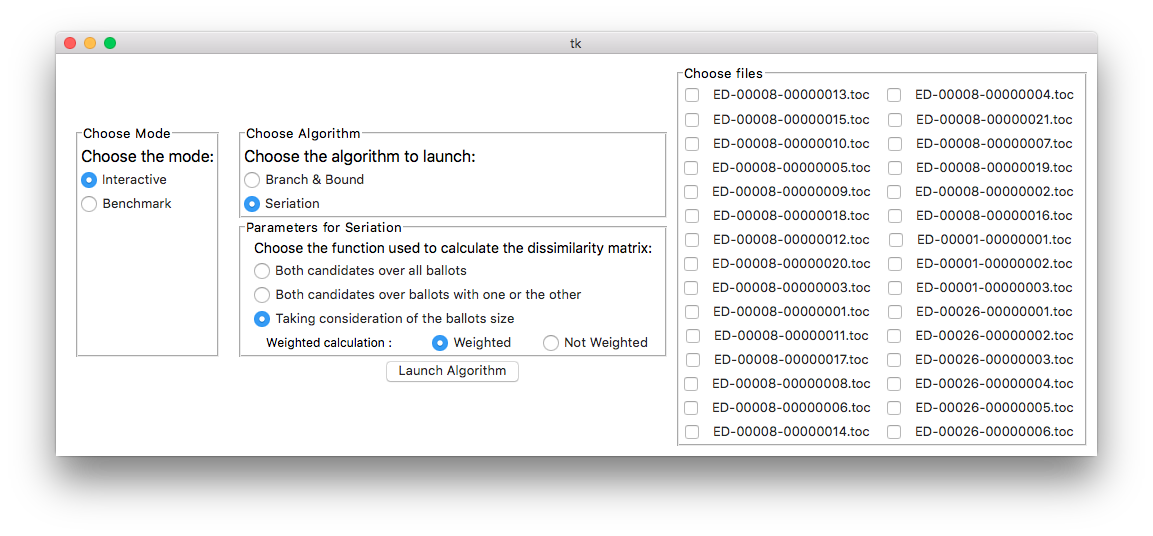
\includegraphics[scale=0.4]{Images/basic-display.png}
\caption{Affichage à l'ouverture du programme}
\end{figure}
\end{center}

Elle comporte deux modes : un mode interactif et un mode \og benchmark \fg. Quel que soit le mode choisi, on a toujours le choix entre les deux algorithmes présentés précédemment. Pour la sériation, un panneau apparaît pour donner le choix entre les 3 fonctions implémentées pour modéliser la dissimilarité entre deux candidats, ainsi que celui du calcul pondéré ou non de la distance à une matrice Anti-Robinson. Pour l'algorithme de branch \& bound, une case apparaît pour donner le choix d'écarter les bulletins que l'on juge non pertinents car ils n'ont recueilli qu'un seul suffrage. Si cette case est cochée, on ne prendra pas en compte les bulletins ayant un nombre de votants égal à 1, et on appliquera l'algorithme sur le reste des bulletins. Enfin, le bouton \og Launch Algorithm \fg{} permet le lancement de l'algorithme choisi sur les fichiers choisis.\\

Dans les deux modes, on choisit toutes les instances sur lesquelles on veut appliquer l'algorithme voulu dans la partie droite de la fenêtre. Cependant l'affichage qui en découle est différent.

\label{graphes-interactif}
Dans le mode \og interactif \fg{}, des graphes simples sont affichés, dans le but de comparer les axes retournés par l'algorithme lancé avec les axes réels. Ils vont permettre de visualiser les erreurs de positionnement rapidement. Il faut tout d'abord récupérer l'axe réel d'une manière ou d'une autre, ici nous avons récupéré les données sur \href{www.wikipedia.fr}{Wikipedia}. Chaque candidat est assimilé à son groupe d'appartenance : extrême gauche, gauche, centre, droite, et extrême droite. En numérotant ces groupes de gauche à droite de 1 à 5, le graphe qui nous permettra de comparer les axes fonctionne comme suit. Il suffit de positionner les candidats sur l'axe des abscisses, et le point correspondant sera l'identifiant du groupe auquel il appartient réellement. Ainsi, si la courbe obtenue est monotone (croissante ou décroissante), l'algorithme aura retourné un axe qui correspond parfaitement à l'axe réel.

\begin{center}
\begin{figure}[H]
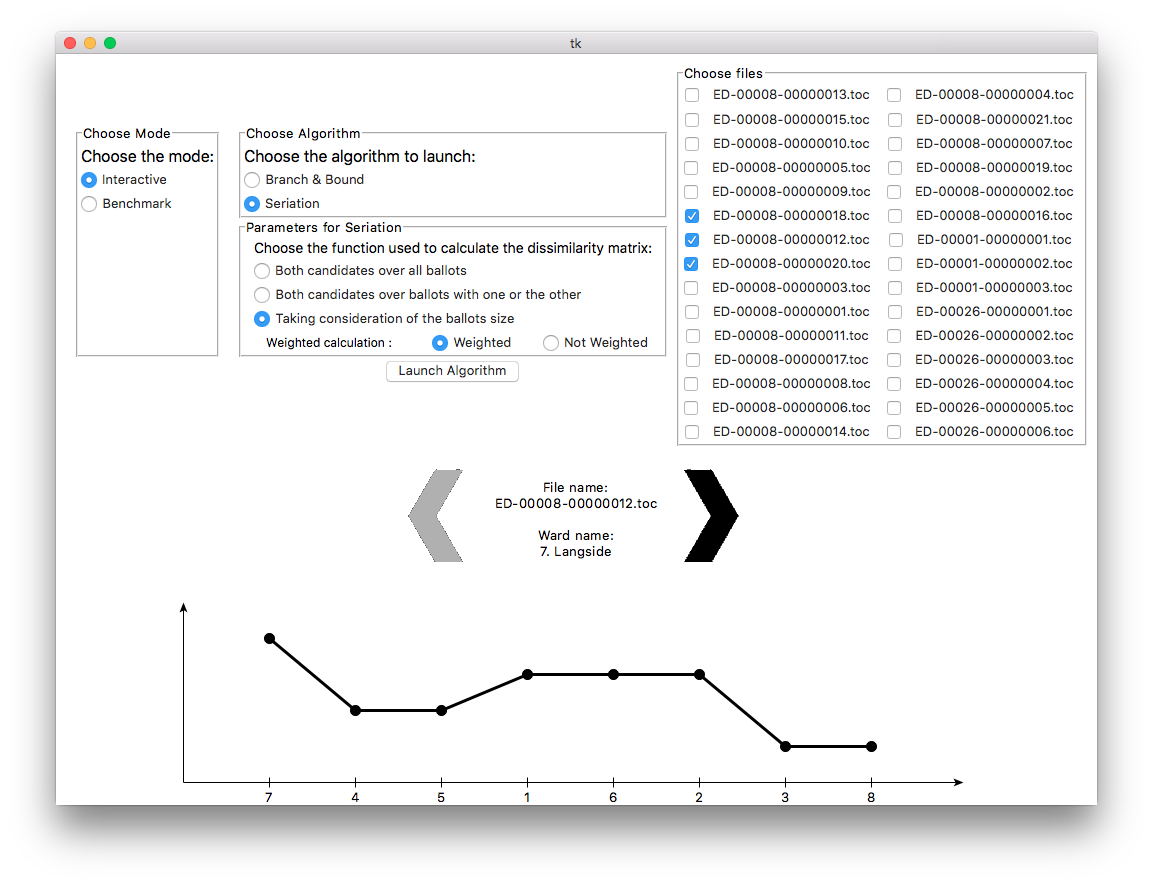
\includegraphics[scale=0.42]{Images/interactive-seriation.png}
\caption{Mode \og interactif \fg{} du programme}
\end{figure}
\end{center}

D'autre part dans le mode \og benchmark \fg, on peut choisir plusieurs fichier sur lesquels lancer l'algorithme choisi. Une fois que l'exécution est terminée sur toutes les instances, un tableau affiche les donneées (nombre total de bulletins et bulletins uniques dans le fichier), les résultats (le nombre d'axes retournés par l'algorithme, ainsi que le nombre total de bulletins sélectionnés et le nombre de bulletins uniques sélectionnés par l'algorithme de branch \& bound) et enfin le temps d'exécution.

\begin{center}
\begin{figure}[H]
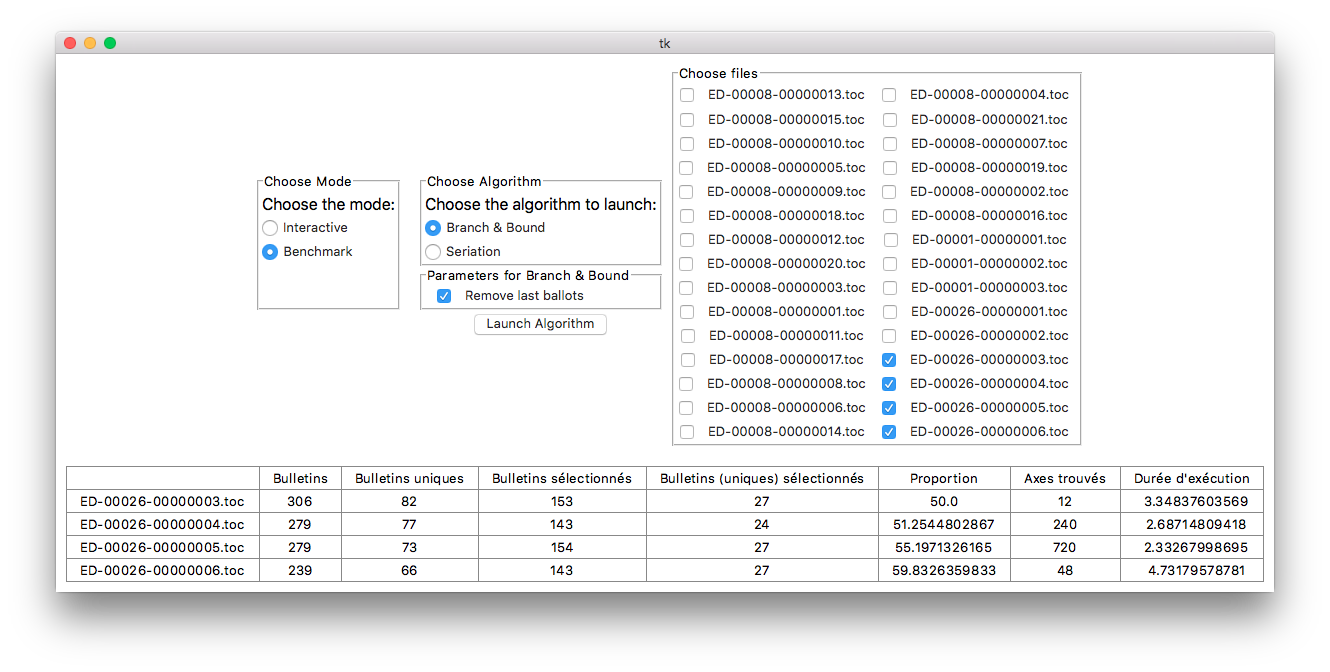
\includegraphics[scale=0.37]{Images/benchmark-bnb.png}
\caption{Mode \og benchmark \fg{} du programme}
\end{figure}
\end{center}

Malheureusement, lorsque l'on clique sur le bouton \og Launch Algorithm \fg{}, comme les algorithmes peuvent prendre un temps assez considérable, toute l'interface se bloque le temps de la résolution. Nous n'avons malheureusement pas eu le temps d'implémenter un système permettant à l'utilisateur de connaître l'avancement des calculs, et de ne pas bloquer entièrement la fenêtre. C'est pourquoi il n'est pas recommandé de lancer le programme sur de nombreux fichiers d'un seul coup.

\subsection{GitHub}
Pour gérer le développement de ce projet en groupe, nous avons utilisé le gestionnaire de version \texttt{git}, avec un dépôt distant sur GitHub. Ce gestionnaire de version est vraiment très pratique pour la gestion des éventuels conflits. De plus, il est très souvent nativement intégré dans les IDE modernes. Enfin, grâce à GitHub, il est très facile de partager le code de notre projet, pour que quiconque y ait accès et puisse suggérer des améliorations.

Notre projet est disponible à cette adresse : \href{https://github.com/lauragreige/P-ANDROIDE}{https://github.com/lauragreige/P-ANDROIDE}.

\section{Exp\'{e}rimentation}

Comme expliqué précédemment, les données utilisées pour réaliser nos tests sont issues du site \href{http://www.preflib.org/}{PrefLib}. Dans cette section, nous allons donner et interpréter certains résultats obtenus avec les différents algorithmes implémentés.

\subsection{Sériation}
%\subsubsection{Temps d'exécution en fonction du nombre de candidats}
Rappelons que la procédure de programmation dynamique est exponentielle en fonction du nombre de candidats qui se présentent à l'élection. En effet, on effectue un appel à cette procédure sur chaque sous-ensemble possible de l'ensemble total de candidat, c'est-à-dire le cardinal de l'ensemble des parties : $2^n$, avec $n$ le cardinal de l'ensemble des candidats. Les différentes circonscriptions et les différentes élections n'ayant pas le même nombre de candidats, ces données vont nous permettre de comparer le temps d'exécution des algorithmes en fonction de ce critère. Voici l'évolution exponentielle du temps de calcul en fonction du nombre de candidats sur la figure suivante :

\begin{figure}[H]
\begin{center}
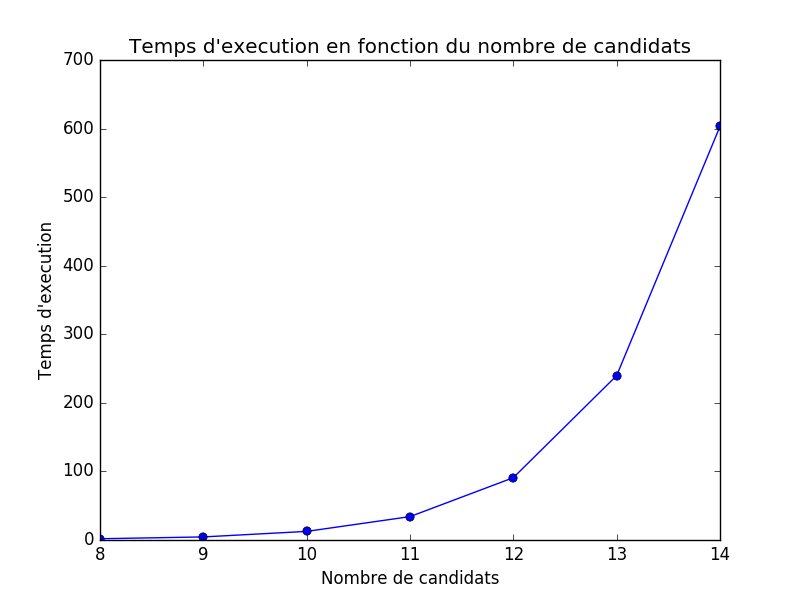
\includegraphics[scale=0.8]{Images/temps-nbCandidats.png}
\caption{Evolution du temps d'exécution en fonction du nombre de candidats}
\end{center}
\end{figure}

%Cela dit, si l'on regarde le temps de calcul nécessaire pour trouver un axe à partir d'une matrice de dissimilarité déjà calculée, celui-ci ne variera que de façon négligeable selon la méthode de calcul de la dissimilarité. 

Le temps d'exécution de l'algorithme de programmation dynamique avec 14 candidats approche les 10 minutes. Au regard de cette évolution très exponentielle, il est donc recommandé de ne pas lancer cet algorithme sur plus d'une quinzaine de candidats. C'est pourquoi, dans ce projet, lorsque nous avons lancé cet algorithme sur les données de l'élection présidentielle française de 2002, y compris depuis l'interface, nous avons retiré les 4 candidats ayant recueilli le moins de suffrage : Corinne Lepage, Daniel Gluckstein, Christiane Taubira, et Christine Boutin. De cette façon, on passe à un problème à 12 candidats, qui se résout en un temps limité.

De plus, le calcul de la matrice de similarité est assez rapide comparé à cette procédure, il est en $O(n^2\times m)$ où $m$ est le nombre de bulletins uniques.
%Donc ce qui va faire la différence, par rapport au temps de calcul, c'est bien le nombre de candidats $n$. Pour le montrer, la figure suivante montre l'évolution du temps d'exécution en fonction de la méthode utilisée pour calculer la dissimilarité entre les candidats. Elle reste quasiment constante :

\bigskip
Comparons maintenant les axes retournés par cette procédure avec les axes réels. Pour cela, nous allons utiliser les graphes décrits dans la section à propos de l'interface (\ref{graphes-interactif}). La monotonie de ces graphes nous informera sur la justesse de notre algorithme.

On peut donc, grâce à ces graphes, comparer les résultats obtenus en fonction de la façon dont on mesure la dissimilarité entre les candidats. Les trois graphes suivants sont les résultats obtenus avec les données issues de l'élection présidentielle française de 2002. Ainsi, les résultats seront encore plus parlants. Ces données recueillies dans 6 bureaux de vote ont été fusionnées pour obtenir des données moins biaisées. Cela dit, toutes ces données proviennent d'une même zone géographique, donc un manque de brassage social peut malheureusement venir biaiser malgré tout nos données. Les graphes décrivant les résultats en fonction des mesures de dissimilarité sont en annexe \ref{resultats-france-seriation}.


On remarque que globalement, quelle que soit la méthode pour mesurer la dissimilarité, les axes trouvés ne sont pas si éloignés de l'axe réel. En effet, à une ou deux inversions près, les courbes sont monotones. Cela s'observe pour toutes les données utilisées lors de ce projet : les données issues des élections irlandaises et de Glasgow. Il y a la plupart du temps de rares inversions dans l'axe, mais les groupes politiques sont le plus souvent assez bien trouvés par l'algorithme. Il arrive même que ce ne soient pas des inversions entre candidats qui soient repérées mais des inversions entre deux groupes entiers. Cela montre bien que la procédure de programmation dynamique implémentée repère bien les candidats qui sont souvent sur le même bulletin. En revanche, entre groupes distincts, comme les votes regroupent rarement des personnes d'affiliation politique très différentes, il est plus difficile de placer ces groupes les uns par rapport aux autres.

De plus, il est intéressant de noter que le plus souvent, c'est en ne pondérant pas le calcul de la distance à une matrice Anti-Robinson qu'on obtient le plus d'axes. En effet, cela est dû au fait qu'en ne pondérant pas nos calculs, il est plus probable que deux matrices donnent le même score final. En revanche si on prend en compte les écarts entre les éléments, donc en pondérant nos calculs, il est fort probable que ces deux matrices aient un score différent l'une de l'autre. Par exemple, pour les données de l'élection présidentielle française de 2002, lors de l'utilisation de la méthode de calcul de dissimilarité \texttt{dissimilarity\_and\_or}, la version pondérée n'a renvoyé qu'un seul axe, alors que la version non-pondérée en a renvoyé 4.

\subsection{Branch \& bound}

L'algorithme de branch \& bound a été appliqué sur les données provenant de l’élection présidentielle française de 2002 seulement (ED-000026-000000XX.toc). En effet, dans le branch \& bound on explore tous les nœuds de l'arbre dans le pire des cas, c'est-à-dire $\sum_{i = 1}^{n} 2^{ i}$ nœuds, $n$ étant le nombre de bulletins uniques. Les données provenant des élections menées en Irlande et à Glasgow contenaient un grand nombre de bulletins uniques (plus de 19000 bulletins uniques pour l'Irlande et plus de 2000 pour Glasgow), il était donc impossible d'appliquer l'algorithme de branch \& bound sur ces données.\\

Dans la suite, on représente chacun des 16 candidats des élections présidentielles françaises par un numéro différent : 1 : Megret, 2 : Lepage, 3 : Gluckstein, 4 : Bayrou, 5 : Chirac, 6 : Le Pen, 7 : Taubira, 8 : Saint-Josse, 9 : Mamere, 10 : Jospin, 11 : Boutin, 12 : Hue, 13 : Chevenement, 14 : Madelin, 15 : Laguillier, 16 : Besancenot.\\

Une fois l'algorithme appliqué sur les données françaises, on affiche les résultats dans le tableau suivant.

\noindent
\begin{figure}[H]
\begin{tabular}{ | p{1.4cm} | r | r | r | r | r |}
\hline
Fichier & Bulletins (dont uniques) & Sélectionnés & Proportion (\%) & Axes trouvés & Durée (en s.)\\ \hline
03.toc & 476 (252) & 171 (45) & 35.9 & 2 & 115.1 \\ \hline
04.toc & 460 (258) & 162 (43) & 35.2 & 1 & 145.9 \\ \hline
05.toc & 472 (266) & 174 (47) & 36.8 & 2 & 908.2 \\ \hline
06.toc & 415 (242) & 161 (45) & 38.8 & 1 & 279.5 \\ \hline
\end{tabular}
\label{BnB-results1}
\caption{Tableau représentant les résultats de l'algorithme de branch \& bound sur les données françaises}
\end{figure}

\noindent La première colonne indique le nombre total de bulletins ainsi que le nombre de bulletins uniques (inscrit entre parenthèses), la deuxième colonne indique le nombre de bulletins sélectionnés ainsi que le nombre de bulletins uniques sélectionnés (inscrit également entre parenthèses). La troisième colonne indique la proportion de bulletins sélectionnés par rapport au nombre total de bulletins et enfin les quatrième et cinquième colonne indiquent respectivement le nombre d'axes trouvés, cohérents avec les bulletins sélectionnés, et la durée d'exécution de l'algorithme.\\

Pour les instances ED-000026-00000001.toc et ED-000026-00000002.toc, le temps d'exécution était trop important par rapport aux autres instances. Nous avons donc implémenté une fonction qui permet d'écarter les bulletins que l'on juge non pertinents (dont le nombre de votants est égal à 1). Ceci nous permet de réduire la taille de l'instance en gardant les bulletins important, afin de diminuer le temps d'exécution. En appliquant cette méthode sur toutes les instances, on obtient les résultats suivants :

\noindent
\begin{figure}[H]
\begin{tabular}{ | p{1.4cm} | r | r | r | r | r |}
\hline
Fichier & Bulletins (dont uniques) & Sélectionnés & Proportion (\%) & Axes trouvés & Durée (en s.)\\ \hline
01.toc & 204 (55) & 129 (25) & 63.2 & 24 & 27.5 \\ \hline
02.toc & 234 (65) & 127 (22) & 54.3 & 720 & 229.9 \\ \hline
03.toc & 306 (82) & 153 (27) & 50.0 & 12 & 3.4 \\ \hline
04.toc & 279 (77) & 143 (24) & 51.3 & 240 & 2.7 \\ \hline
05.toc & 279 (73) & 154 (27) & 55.2 & 720 & 2.3 \\ \hline
06.toc & 239 (66) & 143 (27) & 59.9 & 48 & 4.8 \\ \hline
\end{tabular}
\label{BnB-results2}
\caption{Tableau représentant les résultats de l'algorithme de branch \& bound sur les données françaises en écartant les derniers bulletins}
\end{figure}

\noindent Malheureusement, en écartant les bulletins, on trouve un grand nombre d'axes correspondant au plus large sous-ensemble de bulletins cohérents. Par exemple, avec les données du fichier ED-000026-00000001.toc, on trouve 24 axes possibles : ceci est dû au fait que certains candidats ne figurent pas dans les bulletins non écartés. En effet, si on compare les 24 axes retournés par l'algorithme, on trouve toujours une même séquence de candidats dans les axes, et les candidats ne figurant pas dans les bulletins non écartés se retrouvent de part et d'autre de cette séquence :\\

\begin{figure}[H]
\centering
\begin{tikzpicture}
\draw (-1,0) -- (12,0);
\node[draw,circle, scale=0.7, fill=two] at (0,0) {7};
\node[draw,circle, scale=0.6, fill=two] at (1,0) {16};
\node[draw,circle, scale=0.7, fill=two] at (2,0) {9};
\node[draw,circle, scale=0.6, fill=two] at (3,0) {10};
\node[draw,circle, scale=0.6, fill=two] at (4,0) {12};
\node[draw,circle, scale=0.6, fill=two] at (5,0) {15};
\node[draw,circle, scale=0.7, fill=two] at (6,0) {1};
\node[draw,circle, scale=0.7, fill=two] at (7,0) {6};
\node[draw,circle, scale=0.7, fill=two] at (8,0) {5};
\node[draw,circle, scale=0.7, fill=two] at (9,0) {4};
\node[draw,circle, scale=0.6, fill=two] at (10,0) {14};
\node[draw,circle, scale=0.6, fill=two] at (11,0) {13};
\end{tikzpicture}
\caption{Séquence de l'axe}
\end{figure}

\noindent Les candidats Lepage (2), Gluckstein (3), Saint-Josse (8), Boutin (11) ne figurant pas dans les bulletins ayant servi à construire cet axe, on trouve toutes les permutations possibles de ces candidats de part et d'autre de l'axe. Un exemple d'axe complet obtenu en écartant les bulletins de cette instance :\\

\begin{figure}[H]
\centering
\begin{tikzpicture}
\draw (-4,0) -- (13,0);
\node[draw,circle, scale=0.7, fill=white] at (-3,0) {2};
\node[draw,circle, scale=0.6, fill=white] at (-2,0) {11};
\node[draw,circle, scale=0.7, fill=white] at (-1,0) {3};
\node[draw,circle, scale=0.7, fill=two] at (0,0) {7};
\node[draw,circle, scale=0.6, fill=two] at (1,0) {16};
\node[draw,circle, scale=0.7, fill=two] at (2,0) {9};
\node[draw,circle, scale=0.6, fill=two] at (3,0) {10};
\node[draw,circle, scale=0.6, fill=two] at (4,0) {12};
\node[draw,circle, scale=0.6, fill=two] at (5,0) {15};
\node[draw,circle, scale=0.7, fill=two] at (6,0) {1};
\node[draw,circle, scale=0.7, fill=two] at (7,0) {6};
\node[draw,circle, scale=0.7, fill=two] at (8,0) {5};
\node[draw,circle, scale=0.7, fill=two] at (9,0) {4};
\node[draw,circle, scale=0.6, fill=two] at (10,0) {14};
\node[draw,circle, scale=0.6, fill=two] at (11,0) {13};
\node[draw,circle, scale=0.7, fill=white] at (12,0) {8};
\end{tikzpicture}
\caption{Axe complet}
\end{figure}

\noindent On remarque que lorsqu'on écarte les bulletins, l'axe qu'on obtient n'est pas un axe gauche-droite. En effet, on retrouve Megret (1) et Le Pen (6) vers le centre de l'axe, alors qu'ils font tous les deux partie de l'extrême droite. De plus, si on regarde de plus près les résultats des élections présidentielle de 2002 au 1\ier{} tour, on remarque que Chirac (5) et Le Pen (6) figurent tous les deux sur un même bulletin plusieurs fois, ce qui explique le fait qu'ils soient à côté dans les axes.

\begin{figure}[H]
\centering
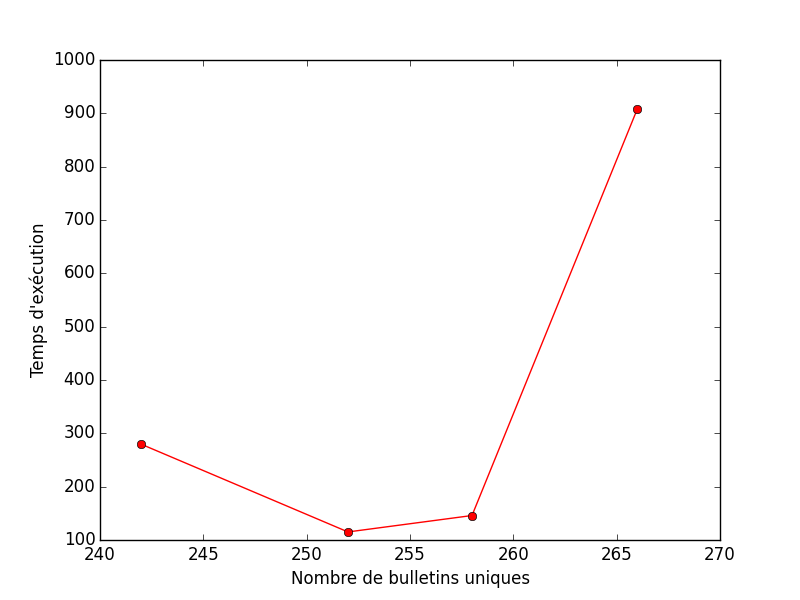
\includegraphics[width=14cm]{Images/graphe_bnb.png}
\label{Graphe:bnb}
\caption{Évolution du temps d'exécution du branche \& bound en fonction du nombre de bulletins uniques}
\end{figure}

Le nombre de nœuds de l'arbre exhaustif des solutions possibles croit très vite lorsque le nombre de bulletins uniques augmente et avec nos tests, on remarque bien que la performance de notre algorithme diffère selon l'instance. La méthode de branch \& bound n'est qu'une construction et un parcours astucieux de cet arbre, qui permet de ne pas explorer certaines branches grâce à un système de minoration et majoration (les bornes inférieures et supérieures) des solutions que cette branche peut produire.

Sur certaines instances le temps d'exécution dépendait plus de la position de la solution optimale dans l'arbre que du nombre de bulletins uniques. En effet, si une solution se trouvait dans la première branche d'un arbre de grande taille, on pourrait obtenir un temps d'exécution qui est inférieur au temps d'exécution d'un arbre de petite taille, dont la solution optimale se trouvait dans une de ses dernières branches. Ceci entraîne donc le parcours de plus de branches de l'arbre, ce qui est tout simplement dû au fait que l'on n'ait pas de \og chance \fg{} sur l'ordre de parcours, et par conséquent, notre algorithme de branch \& bound explorera un très grand ou très petit nombre de nœuds avant de renvoyer la solution optimale quel que soit le nombre de bulletins uniques figurant dans l'instance.\\

Dans la suite, nous étudierons les axes retournés par l'algorithme de branch \& bound sur les instances sans écarter les bulletins. Prenons comme exemple l'axe correspondant aux données du fichier ED-000026-00000003.toc, et comparons celui-ci à l'axe réel.\\

\begin{figure}[H]
\centering
\begin{tikzpicture}
\draw (1,0) -- (18,0);
\node[draw,circle, scale=0.7, fill=one] at (2,0) {3};
\node[draw,circle, scale=0.6, fill=one] at (3,0) {15};
\node[draw,circle, scale=0.6, fill=two] at (4,0) {12};
\node[draw,circle, scale=0.6, fill=one] at (5,0) {16};
\node[draw,circle, scale=0.7, fill=two] at (6,0) {9};
\node[draw,circle, scale=0.6, fill=two] at (7,0) {10};
\node[draw,circle, scale=0.7, fill=two] at (8,0) {7};
\node[draw,circle, scale=0.6, fill=four] at (9,0) {11};
\node[draw,circle, scale=0.7, fill=three] at (10,0) {2};
\node[draw,circle, scale=0.7, fill=three] at (11,0) {4};
\node[draw,circle, scale=0.7, fill=four] at (12,0) {5};
\node[draw,circle, scale=0.6, fill=four] at (13,0) {14};
\node[draw,circle, scale=0.6, fill=two] at (14,0) {13};
\node[draw,circle, scale=0.7, fill=five] at (15,0) {6};
\node[draw,circle, scale=0.7, fill=five] at (16,0) {1};
\node[draw,circle, scale=0.7, fill=four] at (17,0) {8};
\end{tikzpicture}
\caption{Axe branch \& bound}

\vspace{1cm}

\begin{tikzpicture}
\draw (0,0) -- (17,0);
\node[draw,circle, scale=0.7, fill=one] at (1,0) {3};
\node[draw,circle, scale=0.6, fill=one] at (2,0) {15};
\node[draw,circle, scale=0.6, fill=one] at (3,0) {16};
\node[draw,circle, scale=0.7, fill=two] at (4,0) {7};
\node[draw,circle, scale=0.7, fill=two] at (5,0) {9};
\node[draw,circle, scale=0.6, fill=two] at (6,0) {10};
\node[draw,circle, scale=0.6, fill=two] at (7,0) {12};
\node[draw,circle, scale=0.6, fill=two] at (8,0) {13};
\node[draw,circle, scale=0.7, fill=three] at (9,0) {2};
\node[draw,circle, scale=0.7, fill=three] at (10,0) {4};
\node[draw,circle, scale=0.7, fill=four] at (11,0) {5};
\node[draw,circle, scale=0.7, fill=four] at (12,0) {8};
\node[draw,circle, scale=0.6, fill=four] at (13,0) {11};
\node[draw,circle, scale=0.6, fill=four] at (14,0) {14};
\node[draw,circle, scale=0.7, fill=five] at (15,0) {1};
\node[draw,circle, scale=0.7, fill=five] at (16,0) {6};
\end{tikzpicture}
\caption{Axe gauche-droite}
\label{AxeGD}
\end{figure}

Chaque candidat est représenté par une différente nuance de bleu selon son groupe d'appartenance (extrême gauche, gauche, centre, droite et extrême droite) afin de mieux visualiser les similitudes entre les deux axes ainsi que les erreurs de positionnement.

En effet, on retrouve bien les candidats Gluckstein (3), Laguiller (15) et Besancenot (16) à l'extrême gauche, ainsi que Megret (1) et Le Pen (6) à l'extrême droite. De plus, les candidats Taubira (7), Mamere (9), Jospin (10) et Hue (12) sont bien regroupés du même côté de l'axe. De même, les candidats Lepage (2) Bayrou (4), Chirac (5) et Boutin (11) sont regroupés de l'autre côté de l'axe et à la bonne position. Comme pour la sériation, on peut utiliser les graphes pour visualiser les erreurs de positionnement ainsi que les similitudes, pour mieux comparer ces axes à l'axe réel. Les graphes décrivant ces résultats sont en annexe \ref{resultats-france-bnb}.

\section*{Conclusion}
\addcontentsline{toc}{section}{Conclusion}

Dans ce projet, deux approches ont été étudiées et implémentées pour identifier un axe politique gauche-droite à partir de données de votes par approbation. Les deux approches retournent des axes assez proches de l'axe réel et sont globalement correctes. Cependant, en écartant certains bulletins avec la méthode de branch \& bound, on obtient des axes qui ne correspondent pas du tout à la réalité. Le fait de ne pas prendre en compte quelques données que l'on juge non pertinentes et de négliger certains candidats, modifie tout l'axe. Cela dit, on gagne énormément en temps de calcul.

Il est important de noter que ces deux méthodes sont adaptées à deux situations différentes. En effet, le temps d'exécution de la sériation augmente en fonction du nombre de candidats, tandis que celle du branch \& bound augmente en fonction du nombre de bulletins uniques. De plus, le branch \& bound indiquera quels sont les bulletins cohérents ou non avec les axes trouvés. On peut ainsi observer ces incohérences, et déterminer si elles sont le fruit du hasard ou d'une erreur, ou si elles dénotent des idées politiques communes malgré une apparente dissension entre les groupes d'appartenance des candidats impliqués. 

Dans notre cas, l'algorithme de sériation a donné des résultats avec des graphes plus monotones, et donc plus proches de la réalité, que branch \& bound. Cependant, quelle que soit l'algorithme employé, les groupes politiques sont assez bien reconnus et les candidats souvent proches dans l'axe. Les groupes entre eux sont malheureusement parfois interchangés, créant de petites excentricités dans la monotonie. Une étude plus approfondie des différences entre ces deux algorithmes aurait pu être effectuée.

Pour ce projet, il a été nécessaire de réaliser une interface utilisateur pour permettre de lancer les algorithmes et visualiser les axes et les résultats. Notre plus grand regret a été notre incapacité à produire une interface donnant des informations sur le déroulement de l'algorithme lorsqu'il tourne.

\clearpage
\appendix
\section{Annexes}
\subsection{Sériation : Résultats}
\label{resultats-france-seriation}
Ci-dessous sont retranscrits les résultats de l'élection présidentielle française de 2002. Dans les données récupérées, les candidats ont été identifiés de la manière suivante :

\bigskip

\noindent\begin{tabularx}{\textwidth}{XXX}
    1 - Bruno Megret & ~7 - Christiane Taubira & 13 - Jean-Pierre Chevenement\\
    2 - Corinne Lepage & ~8 - Jean Saint-Josse & 14 - Alain Madelin\\
    3 - Daniel Gluckstein & ~9 - Noël Mamere & 15 - Arlette Laguiller\\
    4 - François Bayrou & 10 - Lionel Jospin & 16 - Olivier Besancenot\\
    5 - Jacques Chirac & 11 - Christine Boutin &\\
    6 - LePen & 12 - Robert Hue &\\
\end{tabularx}

\begin{center}
\begin{figure}[H]
\begin{tikzpicture}[x=\textwidth/13, y=\textwidth/13]
\draw[->, >=latex] (0,0) -- (13,0);
\draw[->, >=latex] (0,0) -- (0,5.5);
\draw (1,-0.1) node[below] {8};
\draw (2,-0.1) node[below] {1};
\draw (3,-0.1) node[below] {6};
\draw (4,-0.1) node[below] {14};
\draw (5,-0.1) node[below] {5};
\draw (6,-0.1) node[below] {4};
\draw (7,-0.1) node[below] {13};
\draw (8,-0.1) node[below] {10};
\draw (9,-0.1) node[below] {9};
\draw (10,-0.1) node[below] {16};
\draw (11,-0.1) node[below] {15};
\draw (12,-0.1) node[below] {12};
\draw plot[ultra thick]coordinates{(1,4)(2,5)(3,5)(4,4)(5,4)(6,3)(7,2)(8,2)(9,2)(10,1)(11,1)(12,2)};
\draw[fill=black] (1,4) circle (0.1);
\draw[fill=black] (2,5) circle (0.1);
\draw[fill=black] (3,5) circle (0.1);
\draw[fill=black] (4,4) circle (0.1);
\draw[fill=black] (5,4) circle (0.1);
\draw[fill=black] (6,3) circle (0.1);
\draw[fill=black] (7,2) circle (0.1);
\draw[fill=black] (8,2) circle (0.1);
\draw[fill=black] (9,2) circle (0.1);
\draw[fill=black] (10,1) circle (0.1);
\draw[fill=black] (11,1) circle (0.1);
\draw[fill=black] (12,2) circle (0.1);
\end{tikzpicture}
\caption{Axe trouvé avec dissimilarity\_and\_n et un calcul pondéré}
\end{figure}
\end{center}

\begin{center}
\begin{figure}[H]
\begin{tikzpicture}[x=\textwidth/13, y=\textwidth/13]
\draw[->, >=latex] (0,0) -- (13,0);
\draw[->, >=latex] (0,0) -- (0,5.5);
\draw (1,-0.1) node[below] {1};
\draw (2,-0.1) node[below] {8};
\draw (3,-0.1) node[below] {6};
\draw (4,-0.1) node[below] {14};
\draw (5,-0.1) node[below] {5};
\draw (6,-0.1) node[below] {4};
\draw (7,-0.1) node[below] {13};
\draw (8,-0.1) node[below] {10};
\draw (9,-0.1) node[below] {9};
\draw (10,-0.1) node[below] {15};
\draw (11,-0.1) node[below] {16};
\draw (12,-0.1) node[below] {12};
\draw plot[ultra thick]coordinates{(1,5)(2,4)(3,5)(4,4)(5,4)(6,3)(7,2)(8,2)(9,2)(10,1)(11,1)(12,2)};
\draw[fill=black] (1,5) circle (0.1);
\draw[fill=black] (2,4) circle (0.1);
\draw[fill=black] (3,5) circle (0.1);
\draw[fill=black] (4,4) circle (0.1);
\draw[fill=black] (5,4) circle (0.1);
\draw[fill=black] (6,3) circle (0.1);
\draw[fill=black] (7,2) circle (0.1);
\draw[fill=black] (8,2) circle (0.1);
\draw[fill=black] (9,2) circle (0.1);
\draw[fill=black] (10,1) circle (0.1);
\draw[fill=black] (11,1) circle (0.1);
\draw[fill=black] (12,2) circle (0.1);
\end{tikzpicture}
\caption{Axe trouvé avec dissimilarity\_and\_n et un calcul non-pondéré}
\end{figure}
\end{center}

\begin{center}
\begin{figure}[H]
\begin{tikzpicture}[x=\textwidth/13, y=\textwidth/13]
\draw[->, >=latex] (0,0) -- (13,0);
\draw[->, >=latex] (0,0) -- (0,5.5);
\draw (1,-0.1) node[below] {8};
\draw (2,-0.1) node[below] {1};
\draw (3,-0.1) node[below] {6};
\draw (4,-0.1) node[below] {14};
\draw (5,-0.1) node[below] {5};
\draw (6,-0.1) node[below] {4};
\draw (7,-0.1) node[below] {13};
\draw (8,-0.1) node[below] {10};
\draw (9,-0.1) node[below] {9};
\draw (10,-0.1) node[below] {16};
\draw (11,-0.1) node[below] {15};
\draw (12,-0.1) node[below] {12};
\draw plot[ultra thick]coordinates{(1,4)(2,5)(3,5)(4,4)(5,4)(6,3)(7,2)(8,2)(9,2)(10,1)(11,1)(12,2)};
\draw[fill=black] (1,4) circle (0.1);
\draw[fill=black] (2,5) circle (0.1);
\draw[fill=black] (3,5) circle (0.1);
\draw[fill=black] (4,4) circle (0.1);
\draw[fill=black] (5,4) circle (0.1);
\draw[fill=black] (6,3) circle (0.1);
\draw[fill=black] (7,2) circle (0.1);
\draw[fill=black] (8,2) circle (0.1);
\draw[fill=black] (9,2) circle (0.1);
\draw[fill=black] (10,1) circle (0.1);
\draw[fill=black] (11,1) circle (0.1);
\draw[fill=black] (12,2) circle (0.1);
\end{tikzpicture}
\caption{Axe trouvé avec dissimilarity\_and\_or et un calcul pondéré}
\end{figure}
\end{center}

\begin{center}
\begin{figure}[H]
\begin{tikzpicture}[x=\textwidth/13, y=\textwidth/13]
\draw[->, >=latex] (0,0) -- (13,0);
\draw[->, >=latex] (0,0) -- (0,5.5);
\draw (1,-0.1) node[below] {1};
\draw (2,-0.1) node[below] {6};
\draw (3,-0.1) node[below] {8};
\draw (4,-0.1) node[below] {14};
\draw (5,-0.1) node[below] {5};
\draw (6,-0.1) node[below] {4};
\draw (7,-0.1) node[below] {13};
\draw (8,-0.1) node[below] {10};
\draw (9,-0.1) node[below] {9};
\draw (10,-0.1) node[below] {15};
\draw (11,-0.1) node[below] {16};
\draw (12,-0.1) node[below] {12};
\draw plot[ultra thick]coordinates{(1,5)(2,5)(3,4)(4,4)(5,4)(6,3)(7,2)(8,2)(9,2)(10,1)(11,1)(12,2)};
\draw[fill=black] (1,5) circle (0.1);
\draw[fill=black] (2,5) circle (0.1);
\draw[fill=black] (3,4) circle (0.1);
\draw[fill=black] (4,4) circle (0.1);
\draw[fill=black] (5,4) circle (0.1);
\draw[fill=black] (6,3) circle (0.1);
\draw[fill=black] (7,2) circle (0.1);
\draw[fill=black] (8,2) circle (0.1);
\draw[fill=black] (9,2) circle (0.1);
\draw[fill=black] (10,1) circle (0.1);
\draw[fill=black] (11,1) circle (0.1);
\draw[fill=black] (12,2) circle (0.1);
\end{tikzpicture}
\caption{Axe trouvé avec dissimilarity\_and\_or et un calcul non-pondéré}
\end{figure}
\end{center}

\begin{center}
\begin{figure}[H]
\begin{tikzpicture}[x=\textwidth/13, y=\textwidth/13]
\draw[->, >=latex] (0,0) -- (13,0);
\draw[->, >=latex] (0,0) -- (0,5.5);
\draw (1,-0.1) node[below] {8};
\draw (2,-0.1) node[below] {1};
\draw (3,-0.1) node[below] {6};
\draw (4,-0.1) node[below] {14};
\draw (5,-0.1) node[below] {5};
\draw (6,-0.1) node[below] {4};
\draw (7,-0.1) node[below] {13};
\draw (8,-0.1) node[below] {10};
\draw (9,-0.1) node[below] {9};
\draw (10,-0.1) node[below] {16};
\draw (11,-0.1) node[below] {15};
\draw (12,-0.1) node[below] {12};
\draw plot[ultra thick]coordinates{(1,4)(2,5)(3,5)(4,4)(5,4)(6,3)(7,2)(8,2)(9,2)(10,1)(11,1)(12,2)};
\draw[fill=black] (1,4) circle (0.1);
\draw[fill=black] (2,5) circle (0.1);
\draw[fill=black] (3,5) circle (0.1);
\draw[fill=black] (4,4) circle (0.1);
\draw[fill=black] (5,4) circle (0.1);
\draw[fill=black] (6,3) circle (0.1);
\draw[fill=black] (7,2) circle (0.1);
\draw[fill=black] (8,2) circle (0.1);
\draw[fill=black] (9,2) circle (0.1);
\draw[fill=black] (10,1) circle (0.1);
\draw[fill=black] (11,1) circle (0.1);
\draw[fill=black] (12,2) circle (0.1);
\end{tikzpicture}
\caption{Axe trouvé avec dissimilarity\_over\_over et un calcul pondéré}
\end{figure}
\end{center}

\begin{center}
\begin{figure}[H]
\begin{tikzpicture}[x=\textwidth/13, y=\textwidth/13]
\draw[->, >=latex] (0,0) -- (13,0);
\draw[->, >=latex] (0,0) -- (0,5.5);
\draw (1,-0.1) node[below] {1};
\draw (2,-0.1) node[below] {8};
\draw (3,-0.1) node[below] {6};
\draw (4,-0.1) node[below] {14};
\draw (5,-0.1) node[below] {5};
\draw (6,-0.1) node[below] {4};
\draw (7,-0.1) node[below] {13};
\draw (8,-0.1) node[below] {10};
\draw (9,-0.1) node[below] {9};
\draw (10,-0.1) node[below] {16};
\draw (11,-0.1) node[below] {15};
\draw (12,-0.1) node[below] {12};
\draw plot[ultra thick]coordinates{(1,5)(2,4)(3,5)(4,4)(5,4)(6,3)(7,2)(8,2)(9,2)(10,1)(11,1)(12,2)};
\draw[fill=black] (1,5) circle (0.1);
\draw[fill=black] (2,4) circle (0.1);
\draw[fill=black] (3,5) circle (0.1);
\draw[fill=black] (4,4) circle (0.1);
\draw[fill=black] (5,4) circle (0.1);
\draw[fill=black] (6,3) circle (0.1);
\draw[fill=black] (7,2) circle (0.1);
\draw[fill=black] (8,2) circle (0.1);
\draw[fill=black] (9,2) circle (0.1);
\draw[fill=black] (10,1) circle (0.1);
\draw[fill=black] (11,1) circle (0.1);
\draw[fill=black] (12,2) circle (0.1);
\end{tikzpicture}
\caption{Axe trouvé avec dissimilarity\_over\_over et un calcul pondéré}
\end{figure}
\end{center}

Tous les résultats de l'algorithme de sériation pour les données françaises, irlandaises, et de Glasgow sont disponibles dans notre projet sous \texttt{Data/TeX/pdf}. Nous rappelons que le projet est disponible à cette adresse : \href{https://github.com/lauragreige/P-ANDROIDE}{https://github.com/lauragreige/P-ANDROIDE}.

\subsection{Branch \& bound : Résultats}
\label{resultats-france-bnb}

Ci-dessous les résultats de l'élection présidentielle française de 2002 en utilisant l'algorithme de branch \& bound.\\

\begin{center}
\begin{figure}[H]
\begin{tikzpicture}[x=\textwidth/17, y=\textwidth/17]
\draw[->, >=latex] (0,0) -- (17,0);
\draw[->, >=latex] (0,0) -- (0, 5.5);
\draw (1,-0.1) node[below] {8};
\draw (2,-0.1) node[below] {1};
\draw (3,-0.1) node[below] {6};
\draw (4,-0.1) node[below] {13};
\draw (5,-0.1) node[below] {14};
\draw (6,-0.1) node[below] {5};
\draw (7,-0.1) node[below] {4};
\draw (8,-0.1) node[below] {2};
\draw (9,-0.1) node[below] {11};
\draw (10,-0.1) node[below] {7};
\draw (11,-0.1) node[below] {10};
\draw (12,-0.1) node[below] {9};
\draw (13,-0.1) node[below] {16};
\draw (14,-0.1) node[below] {12};
\draw (15,-0.1) node[below] {15};
\draw (16,-0.1) node[below] {3};
\draw plot[ultra thick]coordinates{(1,4)(2,5)(3,5)(4,2)(5,4)(6,4)(7,3)(8,3)(9,4)(10,2)(11,2)(12,2)(13,1)(14,2)(15,1)(16,1)};
\draw[fill=black] (1,4) circle (0.1);
\draw[fill=black] (2,5) circle (0.1);
\draw[fill=black] (3,5) circle (0.1);
\draw[fill=black] (4,2) circle (0.1);
\draw[fill=black] (5,4) circle (0.1);
\draw[fill=black] (6,4) circle (0.1);
\draw[fill=black] (7,3) circle (0.1);
\draw[fill=black] (8,3) circle (0.1);
\draw[fill=black] (9,4) circle (0.1);
\draw[fill=black] (10,2) circle (0.1);
\draw[fill=black] (11,2) circle (0.1);
\draw[fill=black] (12,2) circle (0.1);
\draw[fill=black] (13,1) circle (0.1);
\draw[fill=black] (14,2) circle (0.1);
\draw[fill=black] (15,1) circle (0.1);
\draw[fill=black] (16,1) circle (0.1);
\end{tikzpicture}
\caption{Axe trouvé avec les données de l'instance ED-00026-00000003.toc}
\end{figure}
\end{center}

\begin{center}
\begin{figure}[H]
\begin{tikzpicture}[x=\textwidth/17, y=\textwidth/17]
\draw[->, >=latex] (0,0) -- (17,0);
\draw[->, >=latex] (0,0) -- (0, 5.5);
\draw (1,-0.1) node[below] {8};
\draw (2,-0.1) node[below] {3};
\draw (3,-0.1) node[below] {7};
\draw (4,-0.1) node[below] {12};
\draw (5,-0.1) node[below] {15};
\draw (6,-0.1) node[below] {16};
\draw (7,-0.1) node[below] {9};
\draw (8,-0.1) node[below] {10};
\draw (9,-0.1) node[below] {13};
\draw (10,-0.1) node[below] {5};
\draw (11,-0.1) node[below] {4};
\draw (12,-0.1) node[below] {14};
\draw (13,-0.1) node[below] {2};
\draw (14,-0.1) node[below] {11};
\draw (15,-0.1) node[below] {6};
\draw (16,-0.1) node[below] {1};
\draw plot[ultra thick]coordinates{(1,4)(2,1)(3,2)(4,2)(5,1)(6,1)(7,2)(8,2)(9,2)(10,4)(11,3)(12,4)(13,3)(14,4)(15,5)(16,5)};
\draw[fill=black] (1,4) circle (0.1);
\draw[fill=black] (2,1) circle (0.1);
\draw[fill=black] (3,2) circle (0.1);
\draw[fill=black] (4,2) circle (0.1);
\draw[fill=black] (5,1) circle (0.1);
\draw[fill=black] (6,1) circle (0.1);
\draw[fill=black] (7,2) circle (0.1);
\draw[fill=black] (8,2) circle (0.1);
\draw[fill=black] (9,2) circle (0.1);
\draw[fill=black] (10,4) circle (0.1);
\draw[fill=black] (11,3) circle (0.1);
\draw[fill=black] (12,4) circle (0.1);
\draw[fill=black] (13,3) circle (0.1);
\draw[fill=black] (14,4) circle (0.1);
\draw[fill=black] (15,5) circle (0.1);
\draw[fill=black] (16,5) circle (0.1);
\end{tikzpicture}
\caption{Axe trouvé avec les données de l'instance ED-00026-00000004.toc}
\end{figure}
\end{center}

\begin{center}
\begin{figure}[H]
\begin{tikzpicture}[x=\textwidth/17, y=\textwidth/17]
\draw[->, >=latex] (0,0) -- (17,0);
\draw[->, >=latex] (0,0) -- (0, 5.5);
\draw (1,-0.1) node[below] {3};
\draw (2,-0.1) node[below] {1};
\draw (3,-0.1) node[below] {11};
\draw (4,-0.1) node[below] {12};
\draw (5,-0.1) node[below] {15};
\draw (6,-0.1) node[below] {16};
\draw (7,-0.1) node[below] {7};
\draw (8,-0.1) node[below] {9};
\draw (9,-0.1) node[below] {10};
\draw (10,-0.1) node[below] {13};
\draw (11,-0.1) node[below] {4};
\draw (12,-0.1) node[below] {5};
\draw (13,-0.1) node[below] {14};
\draw (14,-0.1) node[below] {8};
\draw (15,-0.1) node[below] {2};
\draw (16,-0.1) node[below] {6};
\draw plot[ultra thick]coordinates{(1,1)(2,5)(3,4)(4,2)(5,1)(6,1)(7,2)(8,2)(9,2)(10,2)(11,3)(12,4)(13,4)(14,4)(15,3)(16,5)};
\draw[fill=black] (1,1) circle (0.1);
\draw[fill=black] (2,5) circle (0.1);
\draw[fill=black] (3,4) circle (0.1);
\draw[fill=black] (4,2) circle (0.1);
\draw[fill=black] (5,1) circle (0.1);
\draw[fill=black] (6,1) circle (0.1);
\draw[fill=black] (7,2) circle (0.1);
\draw[fill=black] (8,2) circle (0.1);
\draw[fill=black] (9,2) circle (0.1);
\draw[fill=black] (10,2) circle (0.1);
\draw[fill=black] (11,3) circle (0.1);
\draw[fill=black] (12,4) circle (0.1);
\draw[fill=black] (13,4) circle (0.1);
\draw[fill=black] (14,4) circle (0.1);
\draw[fill=black] (15,3) circle (0.1);
\draw[fill=black] (16,5) circle (0.1);
\end{tikzpicture}
\caption{Axe trouvé avec les données de l'instance ED-00026-00000005.toc}
\end{figure}
\end{center}

\begin{center}
\begin{figure}[H]
\begin{tikzpicture}[x=\textwidth/17, y=\textwidth/17]
\draw[->, >=latex] (0,0) -- (17,0);
\draw[->, >=latex] (0,0) -- (0, 5.5);
\draw (1,-0.1) node[below] {8};
\draw (2,-0.1) node[below] {2};
\draw (3,-0.1) node[below] {14};
\draw (4,-0.1) node[below] {4};
\draw (5,-0.1) node[below] {5};
\draw (6,-0.1) node[below] {6};
\draw (7,-0.1) node[below] {1};
\draw (8,-0.1) node[below] {15};
\draw (9,-0.1) node[below] {12};
\draw (10,-0.1) node[below] {13};
\draw (11,-0.1) node[below] {10};
\draw (12,-0.1) node[below] {9};
\draw (13,-0.1) node[below] {16};
\draw (14,-0.1) node[below] {7};
\draw (15,-0.1) node[below] {3};
\draw (16,-0.1) node[below] {11};
\draw plot[ultra thick]coordinates{(1,4)(2,3)(3,4)(4,3)(5,4)(6,5)(7,5)(8,1)(9,2)(10,2)(11,2)(12,2)(13,1)(14,2)(15,1)(16,4)};
\draw[fill=black] (1,4) circle (0.1);
\draw[fill=black] (2,3) circle (0.1);
\draw[fill=black] (3,4) circle (0.1);
\draw[fill=black] (4,3) circle (0.1);
\draw[fill=black] (5,4) circle (0.1);
\draw[fill=black] (6,5) circle (0.1);
\draw[fill=black] (7,5) circle (0.1);
\draw[fill=black] (8,1) circle (0.1);
\draw[fill=black] (9,2) circle (0.1);
\draw[fill=black] (10,2) circle (0.1);
\draw[fill=black] (11,2) circle (0.1);
\draw[fill=black] (12,2) circle (0.1);
\draw[fill=black] (13,1) circle (0.1);
\draw[fill=black] (14,2) circle (0.1);
\draw[fill=black] (15,1) circle (0.1);
\draw[fill=black] (16,4) circle (0.1);
\end{tikzpicture}
\caption{Axe trouvé avec les données de l'instance ED-00026-00000006.toc}
\end{figure}
\end{center}
%
\bibliographystyle{plain}
\bibliography{rapport}

\end{document}